% Options for packages loaded elsewhere
\PassOptionsToPackage{unicode}{hyperref}
\PassOptionsToPackage{hyphens}{url}
\PassOptionsToPackage{dvipsnames,svgnames,x11names}{xcolor}
%
\documentclass[
  letterpaper,
  DIV=11,
  numbers=noendperiod]{scrartcl}

\usepackage{amsmath,amssymb}
\usepackage{iftex}
\ifPDFTeX
  \usepackage[T1]{fontenc}
  \usepackage[utf8]{inputenc}
  \usepackage{textcomp} % provide euro and other symbols
\else % if luatex or xetex
  \usepackage{unicode-math}
  \defaultfontfeatures{Scale=MatchLowercase}
  \defaultfontfeatures[\rmfamily]{Ligatures=TeX,Scale=1}
\fi
\usepackage{lmodern}
\ifPDFTeX\else  
    % xetex/luatex font selection
\fi
% Use upquote if available, for straight quotes in verbatim environments
\IfFileExists{upquote.sty}{\usepackage{upquote}}{}
\IfFileExists{microtype.sty}{% use microtype if available
  \usepackage[]{microtype}
  \UseMicrotypeSet[protrusion]{basicmath} % disable protrusion for tt fonts
}{}
\makeatletter
\@ifundefined{KOMAClassName}{% if non-KOMA class
  \IfFileExists{parskip.sty}{%
    \usepackage{parskip}
  }{% else
    \setlength{\parindent}{0pt}
    \setlength{\parskip}{6pt plus 2pt minus 1pt}}
}{% if KOMA class
  \KOMAoptions{parskip=half}}
\makeatother
\usepackage{xcolor}
\setlength{\emergencystretch}{3em} % prevent overfull lines
\setcounter{secnumdepth}{-\maxdimen} % remove section numbering
% Make \paragraph and \subparagraph free-standing
\makeatletter
\ifx\paragraph\undefined\else
  \let\oldparagraph\paragraph
  \renewcommand{\paragraph}{
    \@ifstar
      \xxxParagraphStar
      \xxxParagraphNoStar
  }
  \newcommand{\xxxParagraphStar}[1]{\oldparagraph*{#1}\mbox{}}
  \newcommand{\xxxParagraphNoStar}[1]{\oldparagraph{#1}\mbox{}}
\fi
\ifx\subparagraph\undefined\else
  \let\oldsubparagraph\subparagraph
  \renewcommand{\subparagraph}{
    \@ifstar
      \xxxSubParagraphStar
      \xxxSubParagraphNoStar
  }
  \newcommand{\xxxSubParagraphStar}[1]{\oldsubparagraph*{#1}\mbox{}}
  \newcommand{\xxxSubParagraphNoStar}[1]{\oldsubparagraph{#1}\mbox{}}
\fi
\makeatother

\usepackage{color}
\usepackage{fancyvrb}
\newcommand{\VerbBar}{|}
\newcommand{\VERB}{\Verb[commandchars=\\\{\}]}
\DefineVerbatimEnvironment{Highlighting}{Verbatim}{commandchars=\\\{\}}
% Add ',fontsize=\small' for more characters per line
\usepackage{framed}
\definecolor{shadecolor}{RGB}{241,243,245}
\newenvironment{Shaded}{\begin{snugshade}}{\end{snugshade}}
\newcommand{\AlertTok}[1]{\textcolor[rgb]{0.68,0.00,0.00}{#1}}
\newcommand{\AnnotationTok}[1]{\textcolor[rgb]{0.37,0.37,0.37}{#1}}
\newcommand{\AttributeTok}[1]{\textcolor[rgb]{0.40,0.45,0.13}{#1}}
\newcommand{\BaseNTok}[1]{\textcolor[rgb]{0.68,0.00,0.00}{#1}}
\newcommand{\BuiltInTok}[1]{\textcolor[rgb]{0.00,0.23,0.31}{#1}}
\newcommand{\CharTok}[1]{\textcolor[rgb]{0.13,0.47,0.30}{#1}}
\newcommand{\CommentTok}[1]{\textcolor[rgb]{0.37,0.37,0.37}{#1}}
\newcommand{\CommentVarTok}[1]{\textcolor[rgb]{0.37,0.37,0.37}{\textit{#1}}}
\newcommand{\ConstantTok}[1]{\textcolor[rgb]{0.56,0.35,0.01}{#1}}
\newcommand{\ControlFlowTok}[1]{\textcolor[rgb]{0.00,0.23,0.31}{\textbf{#1}}}
\newcommand{\DataTypeTok}[1]{\textcolor[rgb]{0.68,0.00,0.00}{#1}}
\newcommand{\DecValTok}[1]{\textcolor[rgb]{0.68,0.00,0.00}{#1}}
\newcommand{\DocumentationTok}[1]{\textcolor[rgb]{0.37,0.37,0.37}{\textit{#1}}}
\newcommand{\ErrorTok}[1]{\textcolor[rgb]{0.68,0.00,0.00}{#1}}
\newcommand{\ExtensionTok}[1]{\textcolor[rgb]{0.00,0.23,0.31}{#1}}
\newcommand{\FloatTok}[1]{\textcolor[rgb]{0.68,0.00,0.00}{#1}}
\newcommand{\FunctionTok}[1]{\textcolor[rgb]{0.28,0.35,0.67}{#1}}
\newcommand{\ImportTok}[1]{\textcolor[rgb]{0.00,0.46,0.62}{#1}}
\newcommand{\InformationTok}[1]{\textcolor[rgb]{0.37,0.37,0.37}{#1}}
\newcommand{\KeywordTok}[1]{\textcolor[rgb]{0.00,0.23,0.31}{\textbf{#1}}}
\newcommand{\NormalTok}[1]{\textcolor[rgb]{0.00,0.23,0.31}{#1}}
\newcommand{\OperatorTok}[1]{\textcolor[rgb]{0.37,0.37,0.37}{#1}}
\newcommand{\OtherTok}[1]{\textcolor[rgb]{0.00,0.23,0.31}{#1}}
\newcommand{\PreprocessorTok}[1]{\textcolor[rgb]{0.68,0.00,0.00}{#1}}
\newcommand{\RegionMarkerTok}[1]{\textcolor[rgb]{0.00,0.23,0.31}{#1}}
\newcommand{\SpecialCharTok}[1]{\textcolor[rgb]{0.37,0.37,0.37}{#1}}
\newcommand{\SpecialStringTok}[1]{\textcolor[rgb]{0.13,0.47,0.30}{#1}}
\newcommand{\StringTok}[1]{\textcolor[rgb]{0.13,0.47,0.30}{#1}}
\newcommand{\VariableTok}[1]{\textcolor[rgb]{0.07,0.07,0.07}{#1}}
\newcommand{\VerbatimStringTok}[1]{\textcolor[rgb]{0.13,0.47,0.30}{#1}}
\newcommand{\WarningTok}[1]{\textcolor[rgb]{0.37,0.37,0.37}{\textit{#1}}}

\providecommand{\tightlist}{%
  \setlength{\itemsep}{0pt}\setlength{\parskip}{0pt}}\usepackage{longtable,booktabs,array}
\usepackage{calc} % for calculating minipage widths
% Correct order of tables after \paragraph or \subparagraph
\usepackage{etoolbox}
\makeatletter
\patchcmd\longtable{\par}{\if@noskipsec\mbox{}\fi\par}{}{}
\makeatother
% Allow footnotes in longtable head/foot
\IfFileExists{footnotehyper.sty}{\usepackage{footnotehyper}}{\usepackage{footnote}}
\makesavenoteenv{longtable}
\usepackage{graphicx}
\makeatletter
\def\maxwidth{\ifdim\Gin@nat@width>\linewidth\linewidth\else\Gin@nat@width\fi}
\def\maxheight{\ifdim\Gin@nat@height>\textheight\textheight\else\Gin@nat@height\fi}
\makeatother
% Scale images if necessary, so that they will not overflow the page
% margins by default, and it is still possible to overwrite the defaults
% using explicit options in \includegraphics[width, height, ...]{}
\setkeys{Gin}{width=\maxwidth,height=\maxheight,keepaspectratio}
% Set default figure placement to htbp
\makeatletter
\def\fps@figure{htbp}
\makeatother

\KOMAoption{captions}{tableheading}
\makeatletter
\@ifpackageloaded{caption}{}{\usepackage{caption}}
\AtBeginDocument{%
\ifdefined\contentsname
  \renewcommand*\contentsname{Table of contents}
\else
  \newcommand\contentsname{Table of contents}
\fi
\ifdefined\listfigurename
  \renewcommand*\listfigurename{List of Figures}
\else
  \newcommand\listfigurename{List of Figures}
\fi
\ifdefined\listtablename
  \renewcommand*\listtablename{List of Tables}
\else
  \newcommand\listtablename{List of Tables}
\fi
\ifdefined\figurename
  \renewcommand*\figurename{Figure}
\else
  \newcommand\figurename{Figure}
\fi
\ifdefined\tablename
  \renewcommand*\tablename{Table}
\else
  \newcommand\tablename{Table}
\fi
}
\@ifpackageloaded{float}{}{\usepackage{float}}
\floatstyle{ruled}
\@ifundefined{c@chapter}{\newfloat{codelisting}{h}{lop}}{\newfloat{codelisting}{h}{lop}[chapter]}
\floatname{codelisting}{Listing}
\newcommand*\listoflistings{\listof{codelisting}{List of Listings}}
\makeatother
\makeatletter
\makeatother
\makeatletter
\@ifpackageloaded{caption}{}{\usepackage{caption}}
\@ifpackageloaded{subcaption}{}{\usepackage{subcaption}}
\makeatother

\ifLuaTeX
  \usepackage{selnolig}  % disable illegal ligatures
\fi
\usepackage{bookmark}

\IfFileExists{xurl.sty}{\usepackage{xurl}}{} % add URL line breaks if available
\urlstyle{same} % disable monospaced font for URLs
\hypersetup{
  pdftitle={Maize Analysis},
  pdfauthor={Nanyaemuny Savins},
  colorlinks=true,
  linkcolor={blue},
  filecolor={Maroon},
  citecolor={Blue},
  urlcolor={Blue},
  pdfcreator={LaTeX via pandoc}}


\title{Maize Analysis}
\author{Nanyaemuny Savins}
\date{}

\begin{document}
\maketitle


\subsection{Load necessary packages}\label{load-necessary-packages}

\begin{Shaded}
\begin{Highlighting}[]
\FunctionTok{library}\NormalTok{(readxl)}
\FunctionTok{library}\NormalTok{(tidyverse)}
\FunctionTok{library}\NormalTok{(zoo)}
\FunctionTok{library}\NormalTok{(forecast)}
\FunctionTok{library}\NormalTok{(lubridate)}
\FunctionTok{library}\NormalTok{(seasonal)}
\FunctionTok{library}\NormalTok{(moments)}
\end{Highlighting}
\end{Shaded}

\textbf{This notebook aims to cover the following:}

\begin{itemize}
\item
  Load the Different Folders containing the wholesale and retail prices
  of \emph{maize} from different markets in Kenya
\item
  Perform Data cleaning on the Data while ensuring data Integrity in the
  data
\item
  Visualize the different sales prices from different regions of Kenya
\item
  Model a Time series on the data using ARIMA and ETS models to fit on
  the data and forecast the next 5 months of the data.
\end{itemize}

\subsection{Import Data}\label{import-data}

The structure of my data stored in a folder \texttt{Maize}

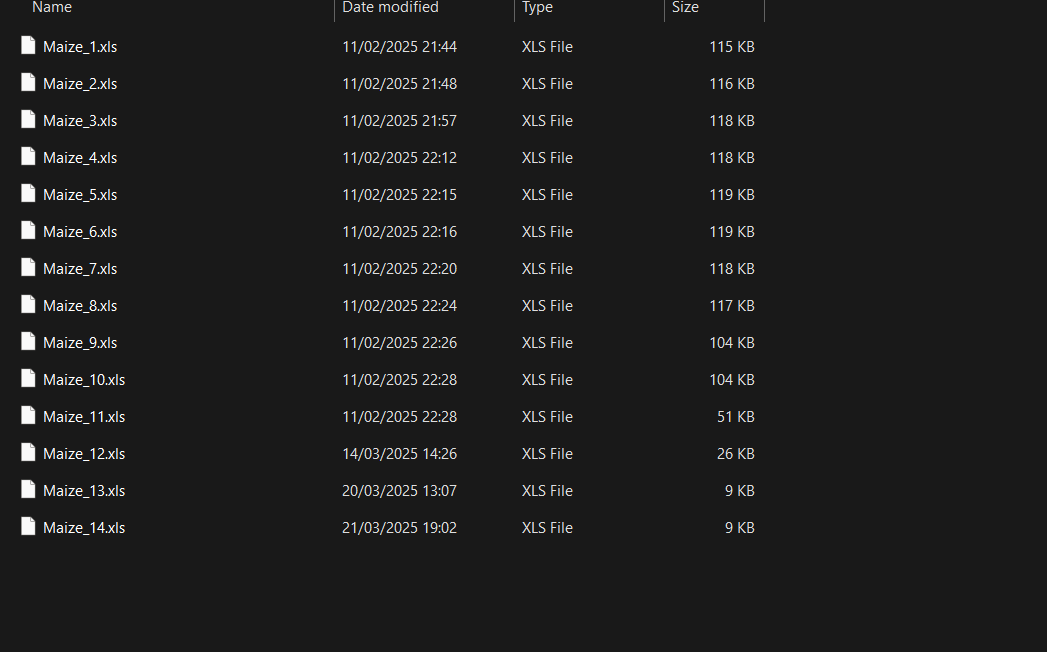
\includegraphics{images/clipboard-1657767075.png}

We need to import the different files and merge them to one dataset
\texttt{maize\_df} . To achieve this we will use a for loop to loop
through the different files and create a list containing the names in
our directory \emph{maize} . Afterwards use the \texttt{map\_df} which
takes in a file list and a function that extract data from each file and
merges them

\begin{Shaded}
\begin{Highlighting}[]
\CommentTok{\# Create a list of file names}
\NormalTok{file\_name }\OtherTok{=} \StringTok{"Maize\_"}
\NormalTok{file\_list }\OtherTok{=}\FunctionTok{list}\NormalTok{()}
\NormalTok{path }\OtherTok{\textless{}{-}} \StringTok{"Maize/"}

\ControlFlowTok{for}\NormalTok{ (i }\ControlFlowTok{in} \DecValTok{1}\SpecialCharTok{:}\DecValTok{14}\NormalTok{)\{}
\NormalTok{  file\_list[[i]] }\OtherTok{\textless{}{-}} \FunctionTok{paste0}\NormalTok{(path,file\_name,i,}\StringTok{\textquotesingle{}.xls\textquotesingle{}}\NormalTok{)}
\NormalTok{\}}

\CommentTok{\# Function to extract the data from a single file}
\NormalTok{extract\_data }\OtherTok{\textless{}{-}} \ControlFlowTok{function}\NormalTok{(file)\{}
\NormalTok{  data}\OtherTok{\textless{}{-}} \FunctionTok{read\_xlsx}\NormalTok{(file)}
  \FunctionTok{return}\NormalTok{(data)}
\NormalTok{\}}

\CommentTok{\# Use map\_df to etract data from multiple files in parallel }

\NormalTok{Maize\_df }\OtherTok{\textless{}{-}} \FunctionTok{map\_df}\NormalTok{(file\_list,extract\_data)}

\FunctionTok{dim}\NormalTok{(Maize\_df) }\CommentTok{\# check the dimensions of our data}
\end{Highlighting}
\end{Shaded}

\begin{verbatim}
[1] 31947    10
\end{verbatim}

\begin{Shaded}
\begin{Highlighting}[]
\FunctionTok{names}\NormalTok{(Maize\_df) }\CommentTok{\# check the columns in the data}
\end{Highlighting}
\end{Shaded}

\begin{verbatim}
 [1] "Commodity"      "Classification" "Grade"          "Sex"           
 [5] "Market"         "Wholesale"      "Retail"         "Supply Volume" 
 [9] "County"         "Date"          
\end{verbatim}

\begin{Shaded}
\begin{Highlighting}[]
\FunctionTok{str}\NormalTok{(Maize\_df) }\CommentTok{\# Investigate the structure of the different columns}
\end{Highlighting}
\end{Shaded}

\begin{verbatim}
tibble [31,947 x 10] (S3: tbl_df/tbl/data.frame)
 $ Commodity     : chr [1:31947] "Dry Maize" "Dry Maize" "Dry Maize" "Dry Maize" ...
 $ Classification: chr [1:31947] "White Maize" "White Maize" "White Maize" "Mixed-Traditional" ...
 $ Grade         : chr [1:31947] "-" "-" "-" "-" ...
 $ Sex           : chr [1:31947] "-" "-" "-" "-" ...
 $ Market        : chr [1:31947] "Isebania Market" "Kerugoya" "Eldoret Main" "Musoli Market" ...
 $ Wholesale     : chr [1:31947] "-" "35.00/Kg" "40.00/Kg" "37.78/Kg" ...
 $ Retail        : chr [1:31947] "40.00/Kg" "60.00/Kg" "50.00/Kg" "41.67/Kg" ...
 $ Supply Volume : num [1:31947] 46000 4500 270 15300 12000 22000 5000 5000 NA 3000 ...
 $ County        : chr [1:31947] "Migori" "Kirinyaga" "Uasin-Gishu" "Kakamega" ...
 $ Date          : chr [1:31947] "2025-02-11" "2025-02-11" "2025-02-11" "2025-02-11" ...
\end{verbatim}

It works ! on to the next step as we can observe from the different
columns we need to perform data cleaning on the different columns :

\begin{enumerate}
\def\labelenumi{\arabic{enumi}.}
\item
  Convert the whole\_sale prices and retail prices into numeric
  variables
\item
  Change the character columns to factor they can be helpful in case we
  would be interested in grouping our data later in the exploratory
  analysis
\item
  The Date column should be in date format \texttt{year-month-date}
\item
  Check for Duplicates in the data and handle them
\item
  Handle missing values in the data
\end{enumerate}

\begin{Shaded}
\begin{Highlighting}[]
\CommentTok{\# step 1: Convert prices to numeric columns}
\NormalTok{Maize\_df }\SpecialCharTok{\%\textgreater{}\%}  \FunctionTok{mutate}\NormalTok{(}\AttributeTok{Wholesale=}\FunctionTok{as.numeric}\NormalTok{(}\FunctionTok{gsub}\NormalTok{(}\StringTok{\textquotesingle{}/Kg\textquotesingle{}}\NormalTok{,}\StringTok{\textquotesingle{}\textquotesingle{}}\NormalTok{,Wholesale)),}
                     \AttributeTok{Retail=}\FunctionTok{as.numeric}\NormalTok{(}\FunctionTok{gsub}\NormalTok{(}\StringTok{\textquotesingle{}/Kg\textquotesingle{}}\NormalTok{,}\StringTok{\textquotesingle{}\textquotesingle{}}\NormalTok{,Retail)))}\OtherTok{{-}\textgreater{}}\NormalTok{cln1}
\end{Highlighting}
\end{Shaded}

\begin{verbatim}
Warning: There were 2 warnings in `mutate()`.
The first warning was:
i In argument: `Wholesale = as.numeric(gsub("/Kg", "", Wholesale))`.
Caused by warning:
! NAs introduced by coercion
i Run `dplyr::last_dplyr_warnings()` to see the 1 remaining warning.
\end{verbatim}

\begin{Shaded}
\begin{Highlighting}[]
\NormalTok{cln1 }\SpecialCharTok{\%\textgreater{}\%} \FunctionTok{select}\NormalTok{(Wholesale,Retail) }\SpecialCharTok{\%\textgreater{}\%} \FunctionTok{summary}\NormalTok{()}
\end{Highlighting}
\end{Shaded}

\begin{verbatim}
   Wholesale           Retail       
 Min.   :   0.01   Min.   :   0.01  
 1st Qu.:  30.00   1st Qu.:  45.00  
 Median :  40.00   Median :  60.00  
 Mean   :  54.40   Mean   :  79.15  
 3rd Qu.:  60.00   3rd Qu.:  80.00  
 Max.   :7000.00   Max.   :9000.00  
 NA's   :4443      NA's   :10421    
\end{verbatim}

Perfect 👌🏿 something to note the prices are assumed to be per kg e.g
\texttt{30.0\ implies\ 1kg\ is\ sold\ at\ ksh30.} If we can just observe
the min and max it's absurd for the prices to be that low or that high
more on this later in the notebook.

\begin{Shaded}
\begin{Highlighting}[]
\CommentTok{\# step 2: Convert the Date to a date format}
\NormalTok{cln1 }\SpecialCharTok{\%\textgreater{}\%} \FunctionTok{mutate}\NormalTok{(}\AttributeTok{Date =} \FunctionTok{as.Date}\NormalTok{(Date))}\OtherTok{{-}\textgreater{}}\NormalTok{ cln2}

\NormalTok{cln2 }\SpecialCharTok{\%\textgreater{}\%} \FunctionTok{select}\NormalTok{(Date) }\SpecialCharTok{\%\textgreater{}\%} \FunctionTok{summary}\NormalTok{()}
\end{Highlighting}
\end{Shaded}

\begin{verbatim}
      Date           
 Min.   :2005-02-01  
 1st Qu.:2021-05-24  
 Median :2022-05-12  
 Mean   :2019-12-31  
 3rd Qu.:2023-05-09  
 Max.   :2025-03-21  
\end{verbatim}

Based on the Time frame in the data we have observations from
\texttt{2005-02-01} to \texttt{2025-03-21}

\begin{Shaded}
\begin{Highlighting}[]
\CommentTok{\# step 3: Convert characters columns to factors}
\NormalTok{cln2 }\SpecialCharTok{\%\textgreater{}\%} \FunctionTok{select\_if}\NormalTok{(is.character)}
\end{Highlighting}
\end{Shaded}

\begin{verbatim}
# A tibble: 31,947 x 6
   Commodity Classification    Grade Sex   Market          County     
   <chr>     <chr>             <chr> <chr> <chr>           <chr>      
 1 Dry Maize White Maize       -     -     Isebania Market Migori     
 2 Dry Maize White Maize       -     -     Kerugoya        Kirinyaga  
 3 Dry Maize White Maize       -     -     Eldoret Main    Uasin-Gishu
 4 Dry Maize Mixed-Traditional -     -     Musoli Market   Kakamega   
 5 Dry Maize White Maize       -     -     Kathonzweni     Makueni    
 6 Dry Maize White Maize       -     -     Ahero           Kisumu     
 7 Dry Maize Mixed-Traditional -     -     Ahero           Kisumu     
 8 Dry Maize Mixed-Traditional -     -     Ahero           Kisumu     
 9 Dry Maize White Maize       -     -     Holo            Kisumu     
10 Dry Maize White Maize       -     -     Kapsabet Market Nandi      
# i 31,937 more rows
\end{verbatim}

\begin{Shaded}
\begin{Highlighting}[]
\NormalTok{cln2 }\SpecialCharTok{\%\textgreater{}\%} \FunctionTok{mutate\_if}\NormalTok{(is.character,as.factor)}\OtherTok{{-}\textgreater{}}\NormalTok{ cln3}
\end{Highlighting}
\end{Shaded}

\begin{Shaded}
\begin{Highlighting}[]
\CommentTok{\#step 4: Check for Duplicates}
\FunctionTok{sum}\NormalTok{(}\FunctionTok{duplicated}\NormalTok{(cln3))}
\end{Highlighting}
\end{Shaded}

\begin{verbatim}
[1] 1903
\end{verbatim}

\begin{Shaded}
\begin{Highlighting}[]
\NormalTok{cln3[}\FunctionTok{duplicated}\NormalTok{(cln3),]}
\end{Highlighting}
\end{Shaded}

\begin{verbatim}
# A tibble: 1,903 x 10
   Commodity Classification  Grade Sex   Market Wholesale Retail `Supply Volume`
   <fct>     <fct>           <fct> <fct> <fct>      <dbl>  <dbl>           <dbl>
 1 Dry Maize Mixed-Traditio~ -     -     Ahero       45     50              5000
 2 Dry Maize White Maize     -     -     Katito      44.4   50              7500
 3 Dry Maize Mixed-Traditio~ -     -     Makut~      40     50                NA
 4 Dry Maize White Maize     -     -     Kisasi      45     55                NA
 5 Dry Maize White Maize     -     -     Kange~      42.2   55                NA
 6 Dry Maize White Maize     -     -     Kimil~      35     40              5000
 7 Dry Maize Mixed-Traditio~ -     -     Tawa        30     35              3000
 8 Dry Maize Mixed-Traditio~ -     -     Tawa        30     35              3000
 9 Dry Maize White Maize     -     -     Miruka      37.8   50             45000
10 Dry Maize White Maize     -     -     Buter~      42.2   45.8            4500
# i 1,893 more rows
# i 2 more variables: County <fct>, Date <date>
\end{verbatim}

\begin{Shaded}
\begin{Highlighting}[]
\CommentTok{\# Drop the duplicates}
\NormalTok{cln3 }\SpecialCharTok{\%\textgreater{}\%} \FunctionTok{distinct}\NormalTok{()}\OtherTok{{-}\textgreater{}}\NormalTok{ cln4}

\CommentTok{\# Confirm no duplicates in the data}
\FunctionTok{sum}\NormalTok{(}\FunctionTok{duplicated}\NormalTok{(cln4))}
\end{Highlighting}
\end{Shaded}

\begin{verbatim}
[1] 0
\end{verbatim}

\begin{Shaded}
\begin{Highlighting}[]
\CommentTok{\# Check the data dimension}
\NormalTok{cln4 }\SpecialCharTok{\%\textgreater{}\%} \FunctionTok{dim}\NormalTok{()}
\end{Highlighting}
\end{Shaded}

\begin{verbatim}
[1] 30044    10
\end{verbatim}

\begin{Shaded}
\begin{Highlighting}[]
\CommentTok{\# Step 5: Handling missing values}
\FunctionTok{colMeans}\NormalTok{(}\FunctionTok{is.na}\NormalTok{(cln4)}\SpecialCharTok{*}\DecValTok{100}\NormalTok{)}
\end{Highlighting}
\end{Shaded}

\begin{verbatim}
     Commodity Classification          Grade            Sex         Market 
     0.0000000      0.0000000      0.0000000      0.0000000      0.0000000 
     Wholesale         Retail  Supply Volume         County           Date 
    11.2534949     30.3787778     39.0427373      0.2862468      0.0000000 
\end{verbatim}

\begin{itemize}
\tightlist
\item
  \texttt{Supply\ volumes} has the highest number of missing values with
  more than 39\% of the data containing missing values followed by
  \texttt{Retail} 30\% , \texttt{Wholesale} 11\% and \texttt{County}
  less than 1\%.
\end{itemize}

To get a better understanding of the missing values in the data we will
look at each column individually

\subsubsection{Wholesale prices}\label{wholesale-prices}

We want to \emph{dive deeper} and see how the whole sale prices is
distributed over time.

\begin{description}
\item[Note]
We will set the wholesales prices per kg not to be less than 30 and
above 100. This values I choose them subjectively based on my knowledge
and research of maize prices from different trusted sources.
\end{description}

\begin{Shaded}
\begin{Highlighting}[]
\CommentTok{\# Investigate wholesale prices}
\NormalTok{cln4 }\SpecialCharTok{\%\textgreater{}\%} \FunctionTok{select}\NormalTok{(Wholesale) }\SpecialCharTok{\%\textgreater{}\%} \FunctionTok{summary}\NormalTok{() }\CommentTok{\#\%\textgreater{}\% filter(Wholesale == )}
\end{Highlighting}
\end{Shaded}

\begin{verbatim}
   Wholesale      
 Min.   :   0.01  
 1st Qu.:  30.00  
 Median :  40.00  
 Mean   :  54.58  
 3rd Qu.:  61.11  
 Max.   :7000.00  
 NA's   :3381     
\end{verbatim}

\begin{Shaded}
\begin{Highlighting}[]
\NormalTok{cln4 }\SpecialCharTok{\%\textgreater{}\%} \FunctionTok{filter}\NormalTok{(Wholesale}\SpecialCharTok{\textgreater{}=}\DecValTok{30} \SpecialCharTok{\&}\NormalTok{ Wholesale}\SpecialCharTok{\textless{}=}\DecValTok{100}\NormalTok{) }\SpecialCharTok{\%\textgreater{}\%} \FunctionTok{summary}\NormalTok{()}
\end{Highlighting}
\end{Shaded}

\begin{verbatim}
     Commodity               Classification  Grade       Sex       
 Dry Maize:20225   -                : 2665   -:20225   -   :20225  
                   IRR              :    1             Male:    0  
                   Mixed-Traditional: 3851                         
                   White Maize      :12384                         
                   Yellow Maize     : 1324                         
                                                                   
                                                                   
             Market        Wholesale          Retail        Supply Volume      
 Nakuru Wakulima: 1159   Min.   : 30.00   Min.   :   0.01   Min.   :        0  
 Nyamakima      :  731   1st Qu.: 35.56   1st Qu.:  47.62   1st Qu.:     1800  
 Eldoret Main   :  699   Median : 47.78   Median :  61.11   Median :     5000  
 Kibuye         :  618   Mean   : 50.75   Mean   :  70.65   Mean   :    29952  
 Aram           :  596   3rd Qu.: 64.44   3rd Qu.:  80.00   3rd Qu.:    10230  
 Gikomba        :  415   Max.   :100.00   Max.   :9000.00   Max.   :100000000  
 (Other)        :16007                    NA's   :3462      NA's   :5934       
       County           Date           
 Nairobi  : 2135   Min.   :2008-07-16  
 Nakuru   : 1279   1st Qu.:2021-12-19  
 Siaya    : 1119   Median :2022-10-11  
 Kirinyaga: 1105   Mean   :2021-08-09  
 Kisumu   : 1088   3rd Qu.:2023-07-11  
 (Other)  :13426   Max.   :2025-03-21  
 NA's     :   73                       
\end{verbatim}

\begin{Shaded}
\begin{Highlighting}[]
\NormalTok{cln4 }\SpecialCharTok{\%\textgreater{}\%} \FunctionTok{filter}\NormalTok{(Wholesale}\SpecialCharTok{\textgreater{}=}\DecValTok{30} \SpecialCharTok{\&}\NormalTok{ Wholesale}\SpecialCharTok{\textless{}=}\DecValTok{100}\NormalTok{) }\OtherTok{{-}\textgreater{}}\NormalTok{trial001}

\FunctionTok{ggplot}\NormalTok{(}\AttributeTok{data =}\NormalTok{ trial001,}\FunctionTok{aes}\NormalTok{(Date,Wholesale))}\SpecialCharTok{+}\FunctionTok{geom\_point}\NormalTok{()}
\end{Highlighting}
\end{Shaded}

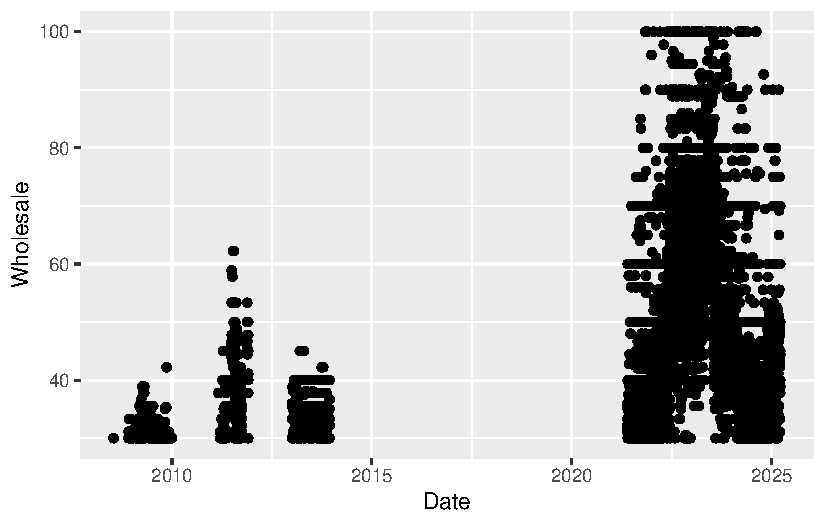
\includegraphics{Maize_analysis_files/figure-pdf/unnamed-chunk-8-1.pdf}

From the scatter plot we can observe we have missing data between 2008
and 2020.This could be caused by few or no observation data collected
for the missing years.

\begin{itemize}
\item
  We will truncate our data and emphasis our analysis on data from 2021
\item
  Missing values for the wholesale prices were removed when filtering
  the wholesale prices
\end{itemize}

\begin{Shaded}
\begin{Highlighting}[]
\NormalTok{trial001 }\SpecialCharTok{\%\textgreater{}\%} \FunctionTok{filter}\NormalTok{(Date }\SpecialCharTok{\textgreater{}} \FunctionTok{as.Date}\NormalTok{(}\StringTok{\textquotesingle{}2020{-}01{-}01\textquotesingle{}}\NormalTok{)) }\OtherTok{{-}\textgreater{}}\NormalTok{trial002}

\FunctionTok{dim}\NormalTok{(trial002)}
\end{Highlighting}
\end{Shaded}

\begin{verbatim}
[1] 17570    10
\end{verbatim}

\begin{Shaded}
\begin{Highlighting}[]
\CommentTok{\# Drop Irrelevant columns}
\NormalTok{trial002 }\SpecialCharTok{\%\textgreater{}\%} \FunctionTok{summary}\NormalTok{()}
\end{Highlighting}
\end{Shaded}

\begin{verbatim}
     Commodity               Classification  Grade       Sex       
 Dry Maize:17570   -                :   10   -:17570   -   :17570  
                   IRR              :    1             Male:    0  
                   Mixed-Traditional: 3851                         
                   White Maize      :12384                         
                   Yellow Maize     : 1324                         
                                                                   
                                                                   
              Market        Wholesale          Retail       
 Nakuru Wakulima :  997   Min.   : 30.00   Min.   :   0.01  
 Nyamakima       :  731   1st Qu.: 38.89   1st Qu.:  47.62  
 Aram            :  596   Median : 50.91   Median :  61.11  
 Eldoret Main    :  451   Mean   : 53.14   Mean   :  70.65  
 Gikomba         :  415   3rd Qu.: 66.67   3rd Qu.:  80.00  
 Ngurubani Market:  322   Max.   :100.00   Max.   :9000.00  
 (Other)         :14058                    NA's   :807      
 Supply Volume             County           Date           
 Min.   :        0   Nairobi  : 1744   Min.   :2021-05-26  
 1st Qu.:     1800   Siaya    : 1118   1st Qu.:2022-05-05  
 Median :     5000   Nakuru   : 1116   Median :2022-12-16  
 Mean   :    29952   Kirinyaga: 1105   Mean   :2023-01-23  
 3rd Qu.:    10230   Kisumu   :  702   3rd Qu.:2023-08-23  
 Max.   :100000000   (Other)  :11712   Max.   :2025-03-21  
 NA's   :3279        NA's     :   73                       
\end{verbatim}

\begin{Shaded}
\begin{Highlighting}[]
\NormalTok{trial002 }\SpecialCharTok{\%\textgreater{}\%} \FunctionTok{select}\NormalTok{(}\SpecialCharTok{{-}}\NormalTok{Commodity,}\SpecialCharTok{{-}}\NormalTok{Grade,}\SpecialCharTok{{-}}\NormalTok{Sex,}\SpecialCharTok{{-}}\StringTok{\textasciigrave{}}\AttributeTok{Supply Volume}\StringTok{\textasciigrave{}}\NormalTok{,}\SpecialCharTok{{-}}\NormalTok{Retail)}\OtherTok{{-}\textgreater{}}\NormalTok{trial003}
\end{Highlighting}
\end{Shaded}

\subsubsection{Exploratory Data
Analysis}\label{exploratory-data-analysis}

\begin{Shaded}
\begin{Highlighting}[]
\NormalTok{trial003}
\end{Highlighting}
\end{Shaded}

\begin{verbatim}
# A tibble: 17,570 x 5
   Classification    Market           Wholesale County      Date      
   <fct>             <fct>                <dbl> <fct>       <date>    
 1 White Maize       Kerugoya              35   Kirinyaga   2025-02-11
 2 White Maize       Eldoret Main          40   Uasin-Gishu 2025-02-11
 3 Mixed-Traditional Musoli Market         37.8 Kakamega    2025-02-11
 4 White Maize       Kathonzweni           45   Makueni     2025-02-11
 5 White Maize       Ahero                 45   Kisumu      2025-02-11
 6 Mixed-Traditional Ahero                 45   Kisumu      2025-02-11
 7 White Maize       Holo                  40   Kisumu      2025-02-11
 8 White Maize       Kapsabet Market       42.2 Nandi       2025-02-11
 9 White Maize       Ngurubani Market      46.7 Kirinyaga   2025-02-11
10 White Maize       Maua                  44.4 Meru        2025-02-11
# i 17,560 more rows
\end{verbatim}

For this section we aim to understand the following from the data:

\begin{enumerate}
\def\labelenumi{\arabic{enumi}.}
\item
  Which counties have data recorded the most and the least wholesale
  prices?
\item
  Which markets have reported the highest and lowest maize prices ?
\item
  Is there significant difference in the prices for the difference
  classes of Dry Maize.?
\end{enumerate}

\begin{Shaded}
\begin{Highlighting}[]
\NormalTok{trial003 }\SpecialCharTok{\%\textgreater{}\%} \FunctionTok{group\_by}\NormalTok{(County) }\SpecialCharTok{\%\textgreater{}\%} \FunctionTok{summarise}\NormalTok{(}\AttributeTok{No.Obs=}\FunctionTok{length}\NormalTok{(Wholesale)) }\SpecialCharTok{\%\textgreater{}\%} \FunctionTok{arrange}\NormalTok{(}\FunctionTok{desc}\NormalTok{(No.Obs)) }\SpecialCharTok{\%\textgreater{}\%} \FunctionTok{head}\NormalTok{(}\DecValTok{10}\NormalTok{) }\OtherTok{{-}\textgreater{}}\NormalTok{pplot}

\FunctionTok{ggplot}\NormalTok{(pplot,}\FunctionTok{aes}\NormalTok{(County,No.Obs)) }\SpecialCharTok{+} \FunctionTok{geom\_col}\NormalTok{(}\FunctionTok{aes}\NormalTok{(}\AttributeTok{fill=}\NormalTok{County))}\SpecialCharTok{+}\FunctionTok{theme}\NormalTok{(}\AttributeTok{legend.position =} \StringTok{\textquotesingle{}none\textquotesingle{}}\NormalTok{)}\SpecialCharTok{+} \FunctionTok{ggtitle}\NormalTok{(}\StringTok{"Top 10 counties observations"}\NormalTok{)}
\end{Highlighting}
\end{Shaded}

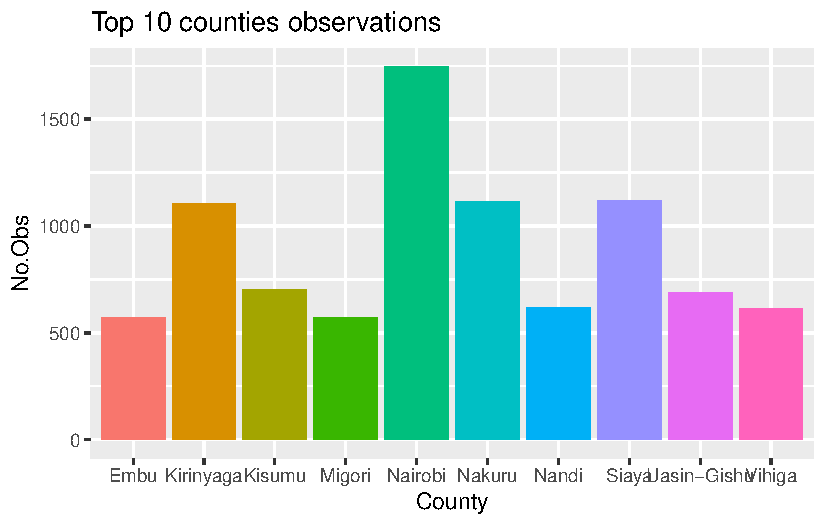
\includegraphics{Maize_analysis_files/figure-pdf/unnamed-chunk-12-1.pdf}

\begin{Shaded}
\begin{Highlighting}[]
\NormalTok{trial003 }\SpecialCharTok{\%\textgreater{}\%} \FunctionTok{group\_by}\NormalTok{(County) }\SpecialCharTok{\%\textgreater{}\%} \FunctionTok{summarise}\NormalTok{(}\AttributeTok{No.Obs=}\FunctionTok{length}\NormalTok{(Wholesale)) }\SpecialCharTok{\%\textgreater{}\%} \FunctionTok{arrange}\NormalTok{(}\FunctionTok{desc}\NormalTok{(No.Obs)) }\SpecialCharTok{\%\textgreater{}\%} \FunctionTok{tail}\NormalTok{(}\DecValTok{10}\NormalTok{) }\OtherTok{{-}\textgreater{}}\NormalTok{pplot}

\FunctionTok{ggplot}\NormalTok{(pplot,}\FunctionTok{aes}\NormalTok{(County,No.Obs)) }\SpecialCharTok{+} \FunctionTok{geom\_col}\NormalTok{(}\FunctionTok{aes}\NormalTok{(}\AttributeTok{fill=}\NormalTok{County))}\SpecialCharTok{+}\FunctionTok{theme}\NormalTok{(}\AttributeTok{legend.position =} \StringTok{\textquotesingle{}none\textquotesingle{}}\NormalTok{)}\SpecialCharTok{+} \FunctionTok{ggtitle}\NormalTok{(}\StringTok{"Bottom 10 counties observations"}\NormalTok{)}
\end{Highlighting}
\end{Shaded}

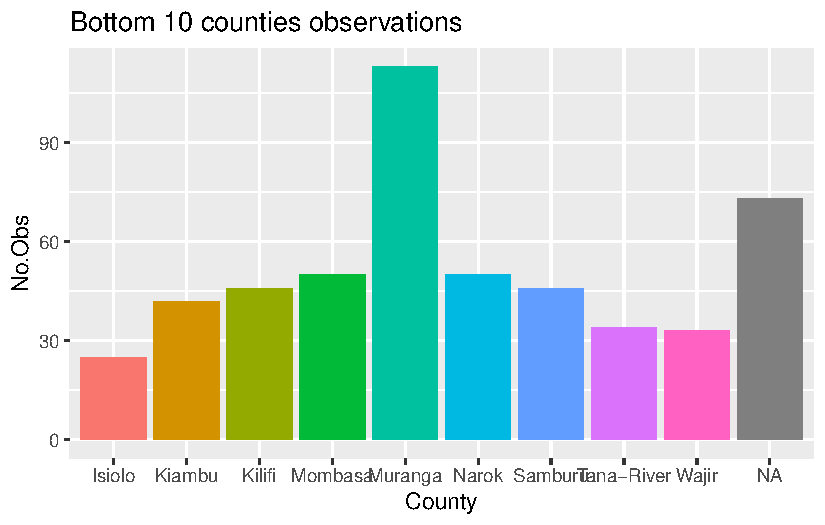
\includegraphics{Maize_analysis_files/figure-pdf/unnamed-chunk-12-2.pdf}

\begin{Shaded}
\begin{Highlighting}[]
\CommentTok{\# What are different means for the wholesale prices for the various counties}
\NormalTok{trial003 }\SpecialCharTok{\%\textgreater{}\%} \FunctionTok{group\_by}\NormalTok{(County,Date) }\SpecialCharTok{\%\textgreater{}\%} \FunctionTok{summarise}\NormalTok{(}\AttributeTok{No.county =}\FunctionTok{length}\NormalTok{(County),}\AttributeTok{Mean\_by\_county =}\FunctionTok{mean}\NormalTok{(Wholesale)) }\SpecialCharTok{\%\textgreater{}\%} \FunctionTok{arrange}\NormalTok{(}\FunctionTok{desc}\NormalTok{(Date))}
\end{Highlighting}
\end{Shaded}

\begin{verbatim}
`summarise()` has grouped output by 'County'. You can override using the
`.groups` argument.
\end{verbatim}

\begin{verbatim}
# A tibble: 12,988 x 4
# Groups:   County [47]
   County        Date       No.county Mean_by_county
   <fct>         <date>         <int>          <dbl>
 1 Bungoma       2025-03-21         1           60  
 2 Busia         2025-03-21         1           70  
 3 Kakamega      2025-03-21         1           37.8
 4 Kirinyaga     2025-03-21         2           39.4
 5 Meru          2025-03-21         1           45  
 6 Nairobi       2025-03-21         1           50  
 7 Tharaka-Nithi 2025-03-21         1           44.4
 8 Kisumu        2025-03-20         1           50  
 9 Nairobi       2025-03-20         1           50  
10 Bungoma       2025-03-19         1           50  
# i 12,978 more rows
\end{verbatim}

\subsubsection{Time series Analysis}\label{time-series-analysis}

\begin{itemize}
\item
  We start of by Investigating skewness in the data this will come in
  handy when trying to identify the best method for aggregating the
  Maize prices.
\item
  Since the prices from different markets are not so skewed we are going
  to use the mean average of the prices in a day as the prices we would
  want to analyse and later work on a model for the data.
\end{itemize}

\begin{Shaded}
\begin{Highlighting}[]
\NormalTok{trial003 }\SpecialCharTok{\%\textgreater{}\%} \FunctionTok{group\_by}\NormalTok{(Date) }\SpecialCharTok{\%\textgreater{}\%} \FunctionTok{summarise}\NormalTok{(}\AttributeTok{Wholesale\_mean =} \FunctionTok{round}\NormalTok{(}\FunctionTok{mean}\NormalTok{(Wholesale),}\DecValTok{2}\NormalTok{))}\OtherTok{{-}\textgreater{}}\NormalTok{ts\_data}

\CommentTok{\# Investigate skewness in the data}
\FunctionTok{ggplot}\NormalTok{(}\AttributeTok{data =}\NormalTok{ ts\_data,}\FunctionTok{aes}\NormalTok{(}\AttributeTok{x=}\NormalTok{Wholesale\_mean))}\SpecialCharTok{+}\FunctionTok{geom\_density}\NormalTok{()}
\end{Highlighting}
\end{Shaded}

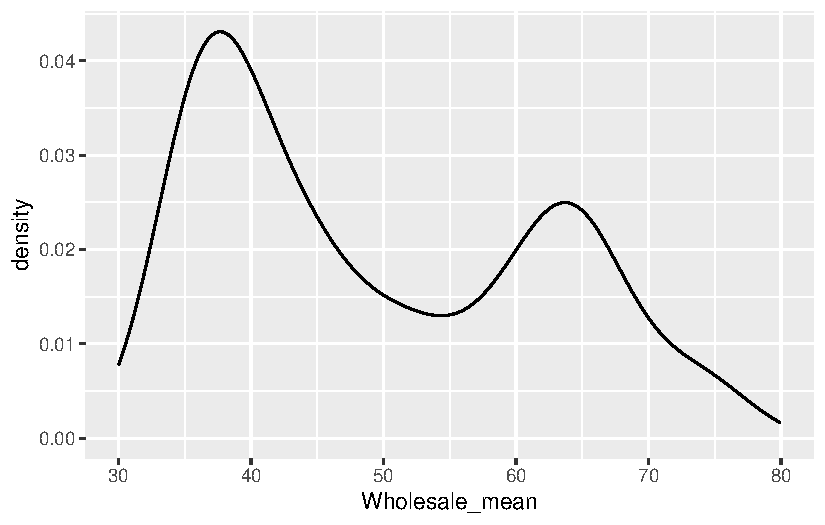
\includegraphics{Maize_analysis_files/figure-pdf/unnamed-chunk-14-1.pdf}

\begin{Shaded}
\begin{Highlighting}[]
\FunctionTok{skewness}\NormalTok{(ts\_data}\SpecialCharTok{$}\NormalTok{Wholesale\_mean)}
\end{Highlighting}
\end{Shaded}

\begin{verbatim}
[1] 0.4354828
\end{verbatim}

We need to convert our data to a time series data something worth
investigating is whether the time series data is irregular. Missing
observations for some days

\begin{Shaded}
\begin{Highlighting}[]
\CommentTok{\# Creating a zoo object}
\NormalTok{Wholesale\_zoo }\OtherTok{\textless{}{-}}\FunctionTok{zoo}\NormalTok{(ts\_data}\SpecialCharTok{$}\NormalTok{Wholesale\_mean,ts\_data}\SpecialCharTok{$}\NormalTok{Date)}

\FunctionTok{length}\NormalTok{(Wholesale\_zoo)}
\end{Highlighting}
\end{Shaded}

\begin{verbatim}
[1] 1378
\end{verbatim}

\begin{Shaded}
\begin{Highlighting}[]
\CommentTok{\# Identifying the missing data}
\NormalTok{full\_dates }\OtherTok{\textless{}{-}} \FunctionTok{seq}\NormalTok{(}\FunctionTok{min}\NormalTok{(ts\_data}\SpecialCharTok{$}\NormalTok{Date),}\FunctionTok{max}\NormalTok{(ts\_data}\SpecialCharTok{$}\NormalTok{Date),}\AttributeTok{by=} \StringTok{\textquotesingle{}day\textquotesingle{}}\NormalTok{)}
\FunctionTok{length}\NormalTok{(full\_dates)}
\end{Highlighting}
\end{Shaded}

\begin{verbatim}
[1] 1396
\end{verbatim}

\begin{Shaded}
\begin{Highlighting}[]
\CommentTok{\# Merge with all dates, introducing NAs for missing dates}
\NormalTok{z\_full }\OtherTok{\textless{}{-}} \FunctionTok{merge.zoo}\NormalTok{(Wholesale\_zoo, }\FunctionTok{zoo}\NormalTok{(, full\_dates), }\AttributeTok{all =} \ConstantTok{TRUE}\NormalTok{)}
\FunctionTok{print}\NormalTok{(z\_full)}
\end{Highlighting}
\end{Shaded}

\begin{verbatim}
2021-05-26 2021-05-27 2021-05-28 2021-05-29 2021-05-30 2021-05-31 2021-06-01 
     33.40      39.44      32.50      34.54         NA      35.29      30.00 
2021-06-02 2021-06-03 2021-06-04 2021-06-05 2021-06-06 2021-06-07 2021-06-08 
     34.66      36.27      34.30      35.42      42.94      32.56      33.89 
2021-06-09 2021-06-10 2021-06-11 2021-06-12 2021-06-13 2021-06-14 2021-06-15 
     31.85      32.78      32.15      33.96      37.72      31.67      36.02 
2021-06-16 2021-06-17 2021-06-18 2021-06-19 2021-06-20 2021-06-21 2021-06-22 
     39.83      36.46      33.44      35.56      35.08      34.53      37.60 
2021-06-23 2021-06-24 2021-06-25 2021-06-26 2021-06-27 2021-06-28 2021-06-29 
     36.83      32.87      33.06      33.61      39.26      34.62      33.70 
2021-06-30 2021-07-01 2021-07-02 2021-07-03 2021-07-04 2021-07-05 2021-07-06 
     37.96      34.63      33.33      31.66      36.90      33.71      33.84 
2021-07-07 2021-07-08 2021-07-09 2021-07-10 2021-07-11 2021-07-12 2021-07-13 
     34.45      34.44      34.11      35.55      35.28      35.78      36.03 
2021-07-14 2021-07-15 2021-07-16 2021-07-17 2021-07-18 2021-07-19 2021-07-20 
     34.49      35.64      33.55      31.56      33.33      35.46      32.56 
2021-07-21 2021-07-22 2021-07-23 2021-07-24 2021-07-25 2021-07-26 2021-07-27 
     33.89      33.55      34.74      32.92      36.67      34.68      33.86 
2021-07-28 2021-07-29 2021-07-30 2021-07-31 2021-08-01 2021-08-02 2021-08-03 
     33.82      36.07      33.09      32.78      32.87      33.40      34.68 
2021-08-04 2021-08-05 2021-08-06 2021-08-07 2021-08-08 2021-08-09 2021-08-10 
     34.00      33.98      34.89      33.08      36.83      33.88      32.45 
2021-08-11 2021-08-12 2021-08-13 2021-08-14 2021-08-15 2021-08-16 2021-08-17 
     37.41      34.59      33.33      32.22      30.56      33.69      34.57 
2021-08-18 2021-08-19 2021-08-20 2021-08-21 2021-08-22 2021-08-23 2021-08-24 
     39.51      33.08      33.47      32.59      35.62      36.68      33.48 
2021-08-25 2021-08-26 2021-08-27 2021-08-28 2021-08-29 2021-08-30 2021-08-31 
     34.88      33.46      36.92      31.85      33.65      33.18      33.52 
2021-09-01 2021-09-02 2021-09-03 2021-09-04 2021-09-05 2021-09-06 2021-09-07 
     33.99      33.08      35.16      31.71      36.80      36.82      33.57 
2021-09-08 2021-09-09 2021-09-10 2021-09-11 2021-09-12 2021-09-13 2021-09-14 
     33.66      35.13      31.93      33.00      35.40      35.23      34.66 
2021-09-15 2021-09-16 2021-09-17 2021-09-18 2021-09-19 2021-09-20 2021-09-21 
     32.54      36.44      34.42      31.85      35.99      34.96      37.49 
2021-09-22 2021-09-23 2021-09-24 2021-09-25 2021-09-26 2021-09-27 2021-09-28 
     34.99      33.69      32.91      40.97      40.00      34.62      34.34 
2021-09-29 2021-09-30 2021-10-01 2021-10-02 2021-10-03 2021-10-04 2021-10-05 
     36.15      36.78      34.81      39.87         NA      36.59      35.12 
2021-10-06 2021-10-07 2021-10-08 2021-10-09 2021-10-10 2021-10-11 2021-10-12 
     39.32      35.62      32.50      35.71      37.61      34.22      37.28 
2021-10-13 2021-10-14 2021-10-15 2021-10-16 2021-10-17 2021-10-18 2021-10-19 
     35.50      36.43      39.35      37.11      30.83      35.11      34.51 
2021-10-20 2021-10-21 2021-10-22 2021-10-23 2021-10-24 2021-10-25 2021-10-26 
     35.04      35.05      38.24      36.66      35.17      35.21      39.90 
2021-10-27 2021-10-28 2021-10-29 2021-10-30 2021-10-31 2021-11-01 2021-11-02 
     35.36      35.31      36.09      35.28      36.85      35.73      34.33 
2021-11-03 2021-11-04 2021-11-05 2021-11-06 2021-11-07 2021-11-08 2021-11-09 
     37.71      37.27      38.65      33.65      34.55      38.36      34.59 
2021-11-10 2021-11-11 2021-11-12 2021-11-13 2021-11-14 2021-11-15 2021-11-16 
     39.86      37.01      44.40      34.28      34.00      34.09      35.17 
2021-11-17 2021-11-18 2021-11-19 2021-11-20 2021-11-21 2021-11-22 2021-11-23 
     37.66      35.81      34.42      38.61      32.87      35.28      34.59 
2021-11-24 2021-11-25 2021-11-26 2021-11-27 2021-11-28 2021-11-29 2021-11-30 
     39.06      40.38      34.80      36.48      57.78      38.85      35.75 
2021-12-01 2021-12-02 2021-12-03 2021-12-04 2021-12-05 2021-12-06 2021-12-07 
     35.11      37.20      34.53      37.46      36.94      37.33      37.65 
2021-12-08 2021-12-09 2021-12-10 2021-12-11 2021-12-12 2021-12-13 2021-12-14 
     36.10      36.44      34.12      35.32      43.33      34.15      34.51 
2021-12-15 2021-12-16 2021-12-17 2021-12-18 2021-12-19 2021-12-20 2021-12-21 
     39.84      35.44      38.02      37.55      32.23      36.83      36.73 
2021-12-22 2021-12-23 2021-12-24 2021-12-25 2021-12-26 2021-12-27 2021-12-28 
     38.80      36.71      40.28      40.00      36.67      35.17      36.27 
2021-12-29 2021-12-30 2021-12-31 2022-01-01 2022-01-02 2022-01-03 2022-01-04 
     36.57      37.30      42.29      34.44      38.89      35.35      37.64 
2022-01-05 2022-01-06 2022-01-07 2022-01-08 2022-01-09 2022-01-10 2022-01-11 
     37.51      35.73      38.50      34.63      34.58      37.88      37.64 
2022-01-12 2022-01-13 2022-01-14 2022-01-15 2022-01-16 2022-01-17 2022-01-18 
     37.59      35.98      37.91      38.15      36.40      40.65      38.11 
2022-01-19 2022-01-20 2022-01-21 2022-01-22 2022-01-23 2022-01-24 2022-01-25 
     37.34      37.82      40.20      35.83      36.09      37.10      37.24 
2022-01-26 2022-01-27 2022-01-28 2022-01-29 2022-01-30 2022-01-31 2022-02-01 
     38.75      37.47      37.25      38.55      36.83      35.40      38.94 
2022-02-02 2022-02-03 2022-02-04 2022-02-05 2022-02-06 2022-02-07 2022-02-08 
     39.68      37.55      37.52      36.88      35.80      35.37      40.03 
2022-02-09 2022-02-10 2022-02-11 2022-02-12 2022-02-13 2022-02-14 2022-02-15 
     39.08      36.39      39.44      39.43      36.48      37.35      37.94 
2022-02-16 2022-02-17 2022-02-18 2022-02-19 2022-02-20 2022-02-21 2022-02-22 
     38.99      38.39      39.47      38.00      38.21      39.20      37.47 
2022-02-23 2022-02-24 2022-02-25 2022-02-26 2022-02-27 2022-02-28 2022-03-01 
     40.22      38.90      38.10      39.24      36.89      38.04      42.06 
2022-03-02 2022-03-03 2022-03-04 2022-03-05 2022-03-06 2022-03-07 2022-03-08 
     38.79      37.21      34.60      38.40      37.94      37.11      41.14 
2022-03-09 2022-03-10 2022-03-11 2022-03-12 2022-03-13 2022-03-14 2022-03-15 
     40.73      41.07      39.33      38.11      39.03      39.26      40.81 
2022-03-16 2022-03-17 2022-03-18 2022-03-19 2022-03-20 2022-03-21 2022-03-22 
     46.37      39.24      36.88      40.67      40.74      37.84      38.82 
2022-03-23 2022-03-24 2022-03-25 2022-03-26 2022-03-27 2022-03-28 2022-03-29 
     47.18      39.98      39.68      41.99      40.06      40.87      38.97 
2022-03-30 2022-03-31 2022-04-01 2022-04-02 2022-04-03 2022-04-04 2022-04-05 
     42.69      40.06      38.36      41.31      37.17      40.57      41.85 
2022-04-06 2022-04-07 2022-04-08 2022-04-09 2022-04-10 2022-04-11 2022-04-12 
     42.55      41.75      38.01      44.20      44.16      42.84      42.05 
2022-04-13 2022-04-14 2022-04-15 2022-04-16 2022-04-17 2022-04-18 2022-04-19 
     42.34      43.12      41.16      47.45      41.63      42.94      40.84 
2022-04-20 2022-04-21 2022-04-22 2022-04-23 2022-04-24 2022-04-25 2022-04-26 
     48.11      44.05      46.40      48.29      46.94      45.59      42.73 
2022-04-27 2022-04-28 2022-04-29 2022-04-30 2022-05-01 2022-05-02 2022-05-03 
     47.52      43.50      44.14      50.04      47.73      43.92      43.28 
2022-05-04 2022-05-05 2022-05-06 2022-05-07 2022-05-08 2022-05-09 2022-05-10 
     48.56      44.09      45.35      49.06      42.72      46.35      45.39 
2022-05-11 2022-05-12 2022-05-13 2022-05-14 2022-05-15 2022-05-16 2022-05-17 
     47.21      46.09      46.64      57.35      48.76      49.74      45.08 
2022-05-18 2022-05-19 2022-05-20 2022-05-21 2022-05-22 2022-05-23 2022-05-24 
     50.26      52.43      49.90      52.44      46.28      50.47      48.41 
2022-05-25 2022-05-26 2022-05-27 2022-05-28 2022-05-29 2022-05-30 2022-05-31 
     49.12      48.22      47.86      51.75      47.91      54.69      50.08 
2022-06-01 2022-06-02 2022-06-03 2022-06-04 2022-06-05 2022-06-06 2022-06-07 
     50.70      52.18      51.26      54.38      47.43      52.33      56.80 
2022-06-08 2022-06-09 2022-06-10 2022-06-11 2022-06-12 2022-06-13 2022-06-14 
     54.67      53.29      51.37      58.24      46.92      56.36      59.03 
2022-06-15 2022-06-16 2022-06-17 2022-06-18 2022-06-19 2022-06-20 2022-06-21 
     59.19      57.80      62.40      63.26      61.85      59.06      69.17 
2022-06-22 2022-06-23 2022-06-24 2022-06-25 2022-06-26 2022-06-27 2022-06-28 
     67.33      66.59      68.07      69.61      68.20      69.87      70.47 
2022-06-29 2022-06-30 2022-07-01 2022-07-02 2022-07-03 2022-07-04 2022-07-05 
     69.42      71.36      68.81      71.39      65.22      67.39      70.15 
2022-07-06 2022-07-07 2022-07-08 2022-07-09 2022-07-10 2022-07-11 2022-07-12 
     70.95      66.30      65.88      75.56      69.63      67.54      69.09 
2022-07-13 2022-07-14 2022-07-15 2022-07-16 2022-07-17 2022-07-18 2022-07-19 
     67.43      74.56      68.80      72.92      67.07      67.73      67.32 
2022-07-20 2022-07-21 2022-07-22 2022-07-23 2022-07-24 2022-07-25 2022-07-26 
     70.80      70.10      65.89      61.48      71.12      62.60      64.97 
2022-07-27 2022-07-28 2022-07-29 2022-07-30 2022-07-31 2022-08-01 2022-08-02 
     67.57      63.29      62.84      64.29      55.87      61.91      64.51 
2022-08-03 2022-08-04 2022-08-05 2022-08-06 2022-08-07 2022-08-08 2022-08-09 
     65.17      63.93      66.05      61.33      69.83      60.56      65.56 
2022-08-10 2022-08-11 2022-08-12 2022-08-13 2022-08-14 2022-08-15 2022-08-16 
     65.62      59.79      60.67      65.67      61.11      63.11      65.42 
2022-08-17 2022-08-18 2022-08-19 2022-08-20 2022-08-21 2022-08-22 2022-08-23 
     65.11      60.02      63.22      66.92      61.59      59.83      61.22 
2022-08-24 2022-08-25 2022-08-26 2022-08-27 2022-08-28 2022-08-29 2022-08-30 
     63.77      61.55      59.17      70.18      58.89      62.00      61.66 
2022-08-31 2022-09-01 2022-09-02 2022-09-03 2022-09-04 2022-09-05 2022-09-06 
     63.06      64.03      60.41      69.74      59.67      60.32      61.95 
2022-09-07 2022-09-08 2022-09-09 2022-09-10 2022-09-11 2022-09-12 2022-09-13 
     61.79      60.86      63.18      63.59      60.34      63.39      63.78 
2022-09-14 2022-09-15 2022-09-16 2022-09-17 2022-09-18 2022-09-19 2022-09-20 
     64.07      60.33      65.91      61.89      56.38      62.38      63.51 
2022-09-21 2022-09-22 2022-09-23 2022-09-24 2022-09-25 2022-09-26 2022-09-27 
     62.14      64.82      65.06      65.79      53.70      64.68      61.63 
2022-09-28 2022-09-29 2022-09-30 2022-10-01 2022-10-02 2022-10-03 2022-10-04 
     64.19      65.39      62.00      65.55      58.82      63.76      64.07 
2022-10-05 2022-10-06 2022-10-07 2022-10-08 2022-10-09 2022-10-10 2022-10-11 
     65.94      66.47      65.64      65.90      59.87      61.84      67.19 
2022-10-12 2022-10-13 2022-10-14 2022-10-15 2022-10-16 2022-10-17 2022-10-18 
     64.87      65.56      64.27      60.06      57.50      64.73      67.52 
2022-10-19 2022-10-20 2022-10-21 2022-10-22 2022-10-23 2022-10-24 2022-10-25 
     65.08      62.86      65.95      62.57      58.67      65.49      64.45 
2022-10-26 2022-10-27 2022-10-28 2022-10-29 2022-10-30 2022-10-31 2022-11-01 
     65.11      65.64      65.51      60.62      63.30      65.71      62.26 
2022-11-02 2022-11-03 2022-11-04 2022-11-05 2022-11-06 2022-11-07 2022-11-08 
     66.72      66.45      63.53      70.97      64.44      64.46      62.41 
2022-11-09 2022-11-10 2022-11-11 2022-11-12 2022-11-13 2022-11-14 2022-11-15 
     63.62      64.27      64.52      58.88      60.45      64.86      62.33 
2022-11-16 2022-11-17 2022-11-18 2022-11-19 2022-11-20 2022-11-21 2022-11-22 
     61.68      64.22      62.88      63.96      60.08      63.44      65.15 
2022-11-23 2022-11-24 2022-11-25 2022-11-26 2022-11-27 2022-11-28 2022-11-29 
     64.59      66.26      65.21      67.03      63.10      64.76      65.85 
2022-11-30 2022-12-01 2022-12-02 2022-12-03 2022-12-04 2022-12-05 2022-12-06 
     63.87      69.63      64.80      60.40      65.33      64.23      61.87 
2022-12-07 2022-12-08 2022-12-09 2022-12-10 2022-12-11 2022-12-12 2022-12-13 
     66.22      65.79      63.74      62.39      67.04      61.16      67.75 
2022-12-14 2022-12-15 2022-12-16 2022-12-17 2022-12-18 2022-12-19 2022-12-20 
     63.77      63.71      62.18      62.44      65.09      64.03      65.03 
2022-12-21 2022-12-22 2022-12-23 2022-12-24 2022-12-25 2022-12-26 2022-12-27 
     64.31      62.23      63.30      64.68         NA      61.75      60.74 
2022-12-28 2022-12-29 2022-12-30 2022-12-31 2023-01-01 2023-01-02 2023-01-03 
     62.71      63.20      60.95      61.94      55.56      62.92      67.39 
2023-01-04 2023-01-05 2023-01-06 2023-01-07 2023-01-08 2023-01-09 2023-01-10 
     65.28      64.00      64.93      62.46      57.19      61.22      63.45 
2023-01-11 2023-01-12 2023-01-13 2023-01-14 2023-01-15 2023-01-16 2023-01-17 
     60.82      59.73      60.57      60.00      60.05      59.98      63.15 
2023-01-18 2023-01-19 2023-01-20 2023-01-21 2023-01-22 2023-01-23 2023-01-24 
     63.93      59.88      56.41      64.11      59.50      58.43      59.76 
2023-01-25 2023-01-26 2023-01-27 2023-01-28 2023-01-29 2023-01-30 2023-01-31 
     59.23      60.97      58.18      57.01      61.93      61.06      62.86 
2023-02-01 2023-02-02 2023-02-03 2023-02-04 2023-02-05 2023-02-06 2023-02-07 
     62.62      59.29      58.81      64.15      54.35      62.14      60.11 
2023-02-08 2023-02-09 2023-02-10 2023-02-11 2023-02-12 2023-02-13 2023-02-14 
     62.21      58.56      61.72      63.33      66.39      62.52      60.09 
2023-02-15 2023-02-16 2023-02-17 2023-02-18 2023-02-19 2023-02-20 2023-02-21 
     62.31      61.40      62.08      66.78      56.66      61.59      64.23 
2023-02-22 2023-02-23 2023-02-24 2023-02-25 2023-02-26 2023-02-27 2023-02-28 
     64.03      65.68      65.88      62.08      58.69      64.91      63.82 
2023-03-01 2023-03-02 2023-03-03 2023-03-04 2023-03-05 2023-03-06 2023-03-07 
     65.87      68.05      66.02      59.46      58.36      65.97      63.97 
2023-03-08 2023-03-09 2023-03-10 2023-03-11 2023-03-12 2023-03-13 2023-03-14 
     65.15      69.99      67.18      66.31      59.65      68.93      68.48 
2023-03-15 2023-03-16 2023-03-17 2023-03-18 2023-03-19 2023-03-20 2023-03-21 
     69.20      71.91      63.04      65.33      55.68      68.91      67.14 
2023-03-22 2023-03-23 2023-03-24 2023-03-25 2023-03-26 2023-03-27 2023-03-28 
     66.70      72.06      65.47      63.23      60.14      69.48      66.82 
2023-03-29 2023-03-30 2023-03-31 2023-04-01 2023-04-02 2023-04-03 2023-04-04 
     68.53      71.48      67.35      71.51      61.41      69.25      68.21 
2023-04-05 2023-04-06 2023-04-07 2023-04-08 2023-04-09 2023-04-10 2023-04-11 
     70.61      69.73      65.89      65.56      65.87      66.60      65.30 
2023-04-12 2023-04-13 2023-04-14 2023-04-15 2023-04-16 2023-04-17 2023-04-18 
     65.18      68.99      64.17      66.78      63.98      68.18      66.01 
2023-04-19 2023-04-20 2023-04-21 2023-04-22 2023-04-23 2023-04-24 2023-04-25 
     66.78      68.83      62.95      66.89      63.37      68.38      66.24 
2023-04-26 2023-04-27 2023-04-28 2023-04-29 2023-04-30 2023-05-01 2023-05-02 
     68.93      66.10      67.94      63.26      62.09      64.45      65.33 
2023-05-03 2023-05-04 2023-05-05 2023-05-06 2023-05-07 2023-05-08 2023-05-09 
     65.87      68.03      66.28      68.79      65.37      68.70      67.09 
2023-05-10 2023-05-11 2023-05-12 2023-05-13 2023-05-14 2023-05-15 2023-05-16 
     70.50      67.86      69.20      74.78      65.76      70.12      70.04 
2023-05-17 2023-05-18 2023-05-19 2023-05-20 2023-05-21 2023-05-22 2023-05-23 
     72.08      74.32      69.98      72.14      67.35      74.57      70.05 
2023-05-24 2023-05-25 2023-05-26 2023-05-27 2023-05-28 2023-05-29 2023-05-30 
     72.06      77.61      74.30      73.40      78.50      74.29      74.26 
2023-05-31 2023-06-01 2023-06-02 2023-06-03 2023-06-04 2023-06-05 2023-06-06 
     74.53      74.92      74.80      73.75      75.17      73.62      73.99 
2023-06-07 2023-06-08 2023-06-09 2023-06-10 2023-06-11 2023-06-12 2023-06-13 
     77.52      74.49      74.04      75.12      78.00      76.65      77.14 
2023-06-14 2023-06-15 2023-06-16 2023-06-17 2023-06-18 2023-06-19 2023-06-20 
     75.78      77.24      75.58      73.68      73.58      75.79      75.98 
2023-06-21 2023-06-22 2023-06-23 2023-06-24 2023-06-25 2023-06-26 2023-06-27 
     74.74      75.18      76.88      71.72      77.73      75.43      74.91 
2023-06-28 2023-06-29 2023-06-30 2023-07-01 2023-07-02 2023-07-03 2023-07-04 
     77.18      72.81      72.95      73.06      79.96      73.47      75.88 
2023-07-05 2023-07-06 2023-07-07 2023-07-08 2023-07-09 2023-07-10 2023-07-11 
     71.99      73.23      76.03      78.12      78.28      72.43      72.74 
2023-07-12 2023-07-13 2023-07-14 2023-07-15 2023-07-16 2023-07-17 2023-07-18 
     74.25      73.63      67.67      69.67      67.46      73.87      72.67 
2023-07-19 2023-07-20 2023-07-21 2023-07-22 2023-07-23 2023-07-24 2023-07-25 
     74.50      65.20      64.48      72.78      69.59      66.73      66.60 
2023-07-26 2023-07-27 2023-07-28 2023-07-29 2023-07-30 2023-07-31 2023-08-01 
     70.37      60.23      62.79      61.22      61.50      63.52      64.84 
2023-08-02 2023-08-03 2023-08-04 2023-08-05 2023-08-06 2023-08-07 2023-08-08 
     62.12      66.45      58.16      61.61      53.67      63.04      62.12 
2023-08-09 2023-08-10 2023-08-11 2023-08-12 2023-08-13 2023-08-14 2023-08-15 
     63.43      62.96      63.12      70.95      52.34      60.22      61.32 
2023-08-16 2023-08-17 2023-08-18 2023-08-19 2023-08-20 2023-08-21 2023-08-22 
     60.35      60.38      59.56      52.78      60.28      58.67      63.22 
2023-08-23 2023-08-24 2023-08-25 2023-08-26 2023-08-27 2023-08-28 2023-08-29 
     58.98      57.78      61.53      57.78      46.74      58.02      62.30 
2023-08-30 2023-08-31 2023-09-01 2023-09-02 2023-09-03 2023-09-04 2023-09-05 
     60.24      58.59      59.17      65.08      54.65      59.08      55.21 
2023-09-06 2023-09-07 2023-09-08 2023-09-09 2023-09-10 2023-09-11 2023-09-12 
     59.24      55.14      60.00      62.36      55.81      58.00      58.44 
2023-09-13 2023-09-14 2023-09-15 2023-09-16 2023-09-17 2023-09-18 2023-09-19 
     57.12      62.70      54.24      51.66      52.13      55.52      57.33 
2023-09-20 2023-09-21 2023-09-22 2023-09-23 2023-09-24 2023-09-25 2023-09-26 
     57.33      61.47      55.43      42.78      47.96      56.90      54.90 
2023-09-27 2023-09-28 2023-09-29 2023-09-30 2023-10-01 2023-10-02 2023-10-03 
     56.76      53.59      58.59      55.56      45.22      59.35      55.47 
2023-10-04 2023-10-05 2023-10-06 2023-10-07 2023-10-08 2023-10-09 2023-10-10 
     53.69      50.69      57.13      49.44      40.84      56.63      44.00 
2023-10-11 2023-10-12 2023-10-13 2023-10-14 2023-10-15 2023-10-16 2023-10-17 
     57.27      47.78      47.33      49.26      41.11      58.93      57.64 
2023-10-18 2023-10-19 2023-10-20 2023-10-21 2023-10-22 2023-10-23 2023-10-24 
     58.70      58.09      51.94      44.44      41.66      55.67      53.80 
2023-10-25 2023-10-26 2023-10-27 2023-10-28 2023-10-29 2023-10-30 2023-10-31 
     56.92      56.67      56.54      47.78      36.00      53.25      54.44 
2023-11-01 2023-11-02 2023-11-03 2023-11-04 2023-11-05 2023-11-06 2023-11-07 
     49.82      55.48      52.95      43.70      50.56      53.06      48.19 
2023-11-08 2023-11-09 2023-11-10 2023-11-11 2023-11-12 2023-11-13 2023-11-14 
     55.00      62.42      49.93      50.00      42.30      42.22      51.30 
2023-11-15 2023-11-16 2023-11-17 2023-11-18 2023-11-19 2023-11-20 2023-11-21 
     46.67      63.13      55.27      46.48      37.25      53.48      51.71 
2023-11-22 2023-11-23 2023-11-24 2023-11-25 2023-11-26 2023-11-27 2023-11-28 
     53.69      52.89      52.64      70.00      42.22      53.83      56.38 
2023-11-29 2023-11-30 2023-12-01 2023-12-02 2023-12-03 2023-12-04 2023-12-05 
     53.69      52.88      51.24      53.33      50.78      54.73      48.94 
2023-12-06 2023-12-07 2023-12-08 2023-12-09 2023-12-10 2023-12-11 2023-12-12 
     48.52      56.08      47.50      44.63         NA      57.14      44.81 
2023-12-13 2023-12-14 2023-12-15 2023-12-16 2023-12-17 2023-12-18 2023-12-19 
     55.46      52.77      50.83      53.33      45.00      52.10      47.81 
2023-12-20 2023-12-21 2023-12-22 2023-12-23 2023-12-24 2023-12-25 2023-12-26 
     51.69      49.56      51.39      44.17      41.11      50.00      52.22 
2023-12-27 2023-12-28 2023-12-29 2023-12-30 2023-12-31 2024-01-01 2024-01-02 
     48.61      52.35      43.16      55.56         NA         NA      50.22 
2024-01-03 2024-01-04 2024-01-05 2024-01-06 2024-01-07 2024-01-08 2024-01-09 
     48.62      52.26      57.38      31.11      36.00      55.62      48.10 
2024-01-10 2024-01-11 2024-01-12 2024-01-13 2024-01-14 2024-01-15 2024-01-16 
     50.18      55.35      49.28      42.22      51.16      52.52      49.49 
2024-01-17 2024-01-18 2024-01-19 2024-01-20 2024-01-21 2024-01-22 2024-01-23 
     49.88      56.60      49.83      60.11      45.83      56.83      50.36 
2024-01-24 2024-01-25 2024-01-26 2024-01-27 2024-01-28 2024-01-29 2024-01-30 
     53.63      52.93      51.34      41.74      38.89      50.99      51.48 
2024-01-31 2024-02-01 2024-02-02 2024-02-03 2024-02-04 2024-02-05 2024-02-06 
     50.90      50.76      46.05      47.50      36.66      49.83      48.82 
2024-02-07 2024-02-08 2024-02-09 2024-02-10 2024-02-11 2024-02-12 2024-02-13 
     52.15      47.26      44.79      52.22      36.00      53.75      48.93 
2024-02-14 2024-02-15 2024-02-16 2024-02-17 2024-02-18 2024-02-19 2024-02-20 
     46.05      46.97      43.59         NA      42.78      44.94      53.03 
2024-02-21 2024-02-22 2024-02-23 2024-02-24 2024-02-25 2024-02-26 2024-02-27 
     45.89      53.17      43.54      44.44      45.84      45.52      45.21 
2024-02-28 2024-02-29 2024-03-01 2024-03-02 2024-03-03 2024-03-04 2024-03-05 
     42.85      51.74      41.87         NA      44.44      45.28      46.16 
2024-03-06 2024-03-07 2024-03-08 2024-03-09 2024-03-10 2024-03-11 2024-03-12 
     44.09      46.07      44.54      45.83      45.00      43.44      47.06 
2024-03-13 2024-03-14 2024-03-15 2024-03-16 2024-03-17 2024-03-18 2024-03-19 
     44.05      51.30      41.05      43.33      43.33      40.97      36.94 
2024-03-20 2024-03-21 2024-03-22 2024-03-23 2024-03-24 2024-03-25 2024-03-26 
     39.48      41.36      42.69      44.44      37.50      46.48      39.67 
2024-03-27 2024-03-28 2024-03-29 2024-03-30 2024-03-31 2024-04-01 2024-04-02 
     42.35      47.96      39.00      30.00      50.00      35.00      49.83 
2024-04-03 2024-04-04 2024-04-05 2024-04-06 2024-04-07 2024-04-08 2024-04-09 
     44.61      35.33      38.52      33.33      39.44      42.10      45.17 
2024-04-10 2024-04-11 2024-04-12 2024-04-13 2024-04-14 2024-04-15 2024-04-16 
     37.11      48.22      40.56      38.78      40.00      39.03      43.57 
2024-04-17 2024-04-18 2024-04-19 2024-04-20 2024-04-21 2024-04-22 2024-04-23 
     39.58      45.89      38.51      33.33         NA      51.72      45.94 
2024-04-24 2024-04-25 2024-04-26 2024-04-27 2024-04-28 2024-04-29 2024-04-30 
     40.76      51.00      38.33      38.52      42.22      43.21      45.53 
2024-05-01 2024-05-02 2024-05-03 2024-05-04 2024-05-05 2024-05-06 2024-05-07 
     36.88      60.74      45.37      34.81      39.89      55.17      44.08 
2024-05-08 2024-05-09 2024-05-10 2024-05-11 2024-05-12 2024-05-13 2024-05-14 
     43.00      54.44      39.84      38.80      36.89      49.69      41.18 
2024-05-15 2024-05-16 2024-05-17 2024-05-18 2024-05-19 2024-05-20 2024-05-21 
        NA         NA         NA         NA         NA      40.00      39.78 
2024-05-22 2024-05-23 2024-05-24 2024-05-25 2024-05-26 2024-05-27 2024-05-28 
     40.69      46.62      38.86      37.43      47.22      47.13      35.93 
2024-05-29 2024-05-30 2024-05-31 2024-06-01 2024-06-02 2024-06-03 2024-06-04 
     39.67      41.40      40.36      37.50      41.25      36.67      39.95 
2024-06-05 2024-06-06 2024-06-07 2024-06-08 2024-06-09 2024-06-10 2024-06-11 
     41.75      40.60      39.18      38.52      43.15      43.56      42.05 
2024-06-12 2024-06-13 2024-06-14 2024-06-15 2024-06-16 2024-06-17 2024-06-18 
     40.65      40.33      38.94      35.92      40.97      40.00      39.02 
2024-06-19 2024-06-20 2024-06-21 2024-06-22 2024-06-23 2024-06-24 2024-06-25 
     36.76      40.56      35.88      36.78      41.67      40.74      37.86 
2024-06-26 2024-06-27 2024-06-28 2024-06-29 2024-06-30 2024-07-01 2024-07-02 
     39.69      40.97      38.02      40.00      38.34      39.51      36.97 
2024-07-03 2024-07-04 2024-07-05 2024-07-06 2024-07-07 2024-07-08 2024-07-09 
     38.72      39.17      38.39      35.56      45.19      41.39      39.77 
2024-07-10 2024-07-11 2024-07-12 2024-07-13 2024-07-14 2024-07-15 2024-07-16 
     39.71      37.49      36.67      37.41      39.44      41.55      37.60 
2024-07-17 2024-07-18 2024-07-19 2024-07-20 2024-07-21 2024-07-22 2024-07-23 
     37.89      40.00      39.52      38.46      39.44      39.50      36.51 
2024-07-24 2024-07-25 2024-07-26 2024-07-27 2024-07-28 2024-07-29 2024-07-30 
     38.74      43.68      35.50      35.00      39.67      38.94      37.48 
2024-07-31 2024-08-01 2024-08-02 2024-08-03 2024-08-04 2024-08-05 2024-08-06 
     36.57      39.20      35.58      33.33      40.00      43.53      36.61 
2024-08-07 2024-08-08 2024-08-09 2024-08-10 2024-08-11 2024-08-12 2024-08-13 
     48.35      41.45      36.85      35.56      41.39      38.03      44.06 
2024-08-14 2024-08-15 2024-08-16 2024-08-17 2024-08-18 2024-08-19 2024-08-20 
     35.94      44.69      35.90      34.81      40.56      34.78      38.02 
2024-08-21 2024-08-22 2024-08-23 2024-08-24 2024-08-25 2024-08-26 2024-08-27 
     38.43      38.29      34.67      34.25      44.00      43.77      37.19 
2024-08-28 2024-08-29 2024-08-30 2024-08-31 2024-09-01 2024-09-02 2024-09-03 
     35.84      38.66      37.80      37.78      40.93      38.54      35.69 
2024-09-04 2024-09-05 2024-09-06 2024-09-07 2024-09-08 2024-09-09 2024-09-10 
     38.33      39.89      36.59      35.89      37.04      37.67      38.99 
2024-09-11 2024-09-12 2024-09-13 2024-09-14 2024-09-15 2024-09-16 2024-09-17 
     38.63      40.83      36.30      35.00      47.08      36.59      34.30 
2024-09-18 2024-09-19 2024-09-20 2024-09-21 2024-09-22 2024-09-23 2024-09-24 
     37.15      38.10      35.10      35.00      35.00      39.67      36.01 
2024-09-25 2024-09-26 2024-09-27 2024-09-28 2024-09-29 2024-09-30 2024-10-01 
     36.71      40.28      35.50      35.00      35.22      39.19      35.98 
2024-10-02 2024-10-03 2024-10-04 2024-10-05 2024-10-06 2024-10-07 2024-10-08 
     36.98      39.49      36.67      32.78      36.54      38.11      37.99 
2024-10-09 2024-10-10 2024-10-11 2024-10-12 2024-10-13 2024-10-14 2024-10-15 
     36.11      39.63      35.76      34.08      34.07      36.81      39.62 
2024-10-16 2024-10-17 2024-10-18 2024-10-19 2024-10-20 2024-10-21 2024-10-22 
     39.39      39.82      35.19      30.00      35.28      47.50      36.04 
2024-10-23 2024-10-24 2024-10-25 2024-10-26 2024-10-27 2024-10-28 2024-10-29 
     38.89      38.56      35.11      37.22      37.78      40.68      35.84 
2024-10-30 2024-10-31 2024-11-01 2024-11-02 2024-11-03 2024-11-04 2024-11-05 
     36.96      43.00      37.30      32.22      37.03      36.30      36.36 
2024-11-06 2024-11-07 2024-11-08 2024-11-09 2024-11-10 2024-11-11 2024-11-12 
     42.28      38.52      36.75      35.93      35.56      38.43      38.00 
2024-11-13 2024-11-14 2024-11-15 2024-11-16 2024-11-17 2024-11-18 2024-11-19 
     41.53      37.29      37.43         NA      36.39      40.32      38.45 
2024-11-20 2024-11-21 2024-11-22 2024-11-23 2024-11-24 2024-11-25 2024-11-26 
     41.08      35.74      37.88         NA      39.63      36.93      39.29 
2024-11-27 2024-11-28 2024-11-29 2024-11-30 2024-12-01 2024-12-02 2024-12-03 
     39.92      36.20      39.23      40.37      42.50      40.00      39.87 
2024-12-04 2024-12-05 2024-12-06 2024-12-07 2024-12-08 2024-12-09 2024-12-10 
     45.17      41.76      41.06      41.11      38.28      41.22      41.27 
2024-12-11 2024-12-12 2024-12-13 2024-12-14 2024-12-15 2024-12-16 2024-12-17 
     44.09      42.22      38.17      42.18      40.56      44.63      40.30 
2024-12-18 2024-12-19 2024-12-20 2024-12-21 2024-12-22 2024-12-23 2024-12-24 
     40.56      41.48      37.54      43.34      40.56      43.89      38.40 
2024-12-25 2024-12-26 2024-12-27 2024-12-28 2024-12-29 2024-12-30 2024-12-31 
     30.00      44.44      34.54      43.61      40.84      42.11      40.08 
2025-01-01 2025-01-02 2025-01-03 2025-01-04 2025-01-05 2025-01-06 2025-01-07 
        NA      39.72      46.22      45.84      45.56      43.89      44.95 
2025-01-08 2025-01-09 2025-01-10 2025-01-11 2025-01-12 2025-01-13 2025-01-14 
     41.22      47.78      45.69      45.00      49.44      47.46      41.25 
2025-01-15 2025-01-16 2025-01-17 2025-01-18 2025-01-19 2025-01-20 2025-01-21 
     42.29      42.78      47.56      43.22      53.78      44.76      43.76 
2025-01-22 2025-01-23 2025-01-24 2025-01-25 2025-01-26 2025-01-27 2025-01-28 
     41.30      47.25      48.81      44.37      40.00      46.81      42.52 
2025-01-29 2025-01-30 2025-01-31 2025-02-01 2025-02-02 2025-02-03 2025-02-04 
     40.06      47.06      45.73      36.67      64.44      44.88      43.15 
2025-02-05 2025-02-06 2025-02-07 2025-02-08 2025-02-09 2025-02-10 2025-02-11 
     44.03      50.71      43.73      45.28      50.89      43.96      41.48 
2025-02-12 2025-02-13 2025-02-14 2025-02-15 2025-02-16 2025-02-17 2025-02-18 
     43.06      43.06      43.45      42.78      45.78      44.18      44.08 
2025-02-19 2025-02-20 2025-02-21 2025-02-22 2025-02-23 2025-02-24 2025-02-25 
     44.10      45.67      44.52      38.06      44.07      47.92      41.59 
2025-02-26 2025-02-27 2025-02-28 2025-03-01 2025-03-02 2025-03-03 2025-03-04 
     43.65      48.01      41.89         NA      40.00      45.83      44.32 
2025-03-05 2025-03-06 2025-03-07 2025-03-08 2025-03-09 2025-03-10 2025-03-11 
     44.99      51.84      41.53      41.43      41.66      52.36      43.78 
2025-03-12 2025-03-13 2025-03-14 2025-03-15 2025-03-16 2025-03-17 2025-03-18 
     43.47      51.11      48.41      38.15      43.56      46.56      42.50 
2025-03-19 2025-03-20 2025-03-21 
     44.09      50.00      48.26 
\end{verbatim}

\begin{Shaded}
\begin{Highlighting}[]
\CommentTok{\# Using Linear Interpolation to fill in missing values}
\NormalTok{Wholesale\_day\_avg }\OtherTok{\textless{}{-}} \FunctionTok{na.approx}\NormalTok{(z\_full)}

\CommentTok{\# Plot the interpolated data}
\FunctionTok{autoplot}\NormalTok{(Wholesale\_day\_avg)}
\end{Highlighting}
\end{Shaded}

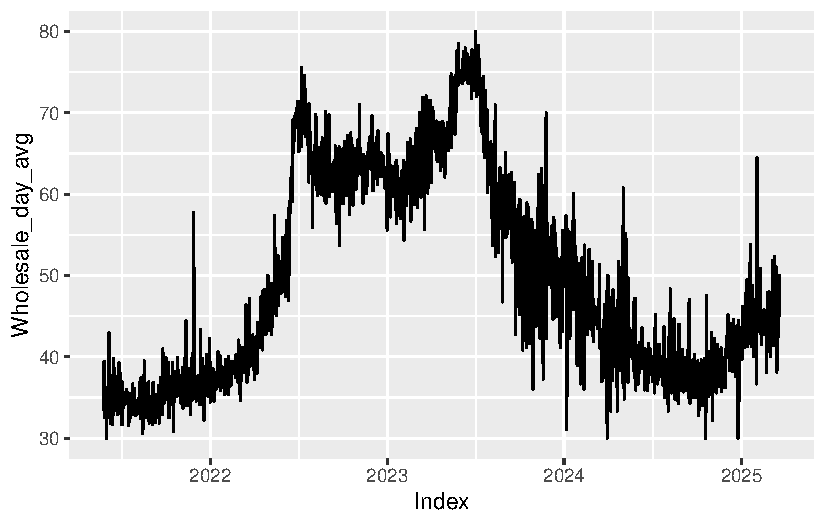
\includegraphics{Maize_analysis_files/figure-pdf/unnamed-chunk-15-1.pdf}

\begin{Shaded}
\begin{Highlighting}[]
\CommentTok{\# Check if the data is irregular}
\FunctionTok{is.regular}\NormalTok{(Wholesale\_day\_avg) }
\end{Highlighting}
\end{Shaded}

\begin{verbatim}
[1] TRUE
\end{verbatim}

\begin{Shaded}
\begin{Highlighting}[]
\NormalTok{Wholesale\_day\_avg }\SpecialCharTok{\%\textgreater{}\%} \FunctionTok{tail}\NormalTok{()}
\end{Highlighting}
\end{Shaded}

\begin{verbatim}
2025-03-16 2025-03-17 2025-03-18 2025-03-19 2025-03-20 2025-03-21 
     43.56      46.56      42.50      44.09      50.00      48.26 
\end{verbatim}

\subsubsection{Smoothing Monthly}\label{smoothing-monthly}

From the plot it is evident linear interpolation does really work well
with our data but we could smooth the data . A different approach to
this we could aggregate the data further into monthly prices for the
wholesale data to see if the data can be smoother.

\begin{Shaded}
\begin{Highlighting}[]
\NormalTok{Wholesale\_month\_avg }\OtherTok{\textless{}{-}}\FunctionTok{aggregate}\NormalTok{(Wholesale\_zoo,as.yearmon,mean)}
\NormalTok{Wholesale\_month\_avg}
\end{Highlighting}
\end{Shaded}

\begin{verbatim}
May 2021 Jun 2021 Jul 2021 Aug 2021 Sep 2021 Oct 2021 Nov 2021 Dec 2021 
35.03400 35.02000 34.27000 34.13935 34.94267 36.05500 37.19967 36.99645 
Jan 2022 Feb 2022 Mar 2022 Apr 2022 May 2022 Jun 2022 Jul 2022 Aug 2022 
37.20806 38.17857 39.92355 43.38700 48.29484 59.95367 67.56645 63.17516 
Sep 2022 Oct 2022 Nov 2022 Dec 2022 Jan 2023 Feb 2023 Mar 2023 Apr 2023 
62.56400 63.88774 64.07500 63.74700 61.03097 62.01536 65.99548 66.49967 
May 2023 Jun 2023 Jul 2023 Aug 2023 Sep 2023 Oct 2023 Nov 2023 Dec 2023 
70.56806 75.21233 70.44903 60.11452 56.47167 51.53806 51.63800 50.16621 
Jan 2024 Feb 2024 Mar 2024 Apr 2024 May 2024 Jun 2024 Jul 2024 Aug 2024 
49.69500 46.79571 43.18933 41.55655 42.91808 39.57600 38.75613 38.68774 
Sep 2024 Oct 2024 Nov 2024 Dec 2024 Jan 2025 Feb 2025 Mar 2025 
37.54067 37.35097 37.94143 40.83161 44.86933 44.82464 45.19250 
\end{verbatim}

\begin{Shaded}
\begin{Highlighting}[]
\FunctionTok{autoplot}\NormalTok{(Wholesale\_month\_avg)}
\end{Highlighting}
\end{Shaded}

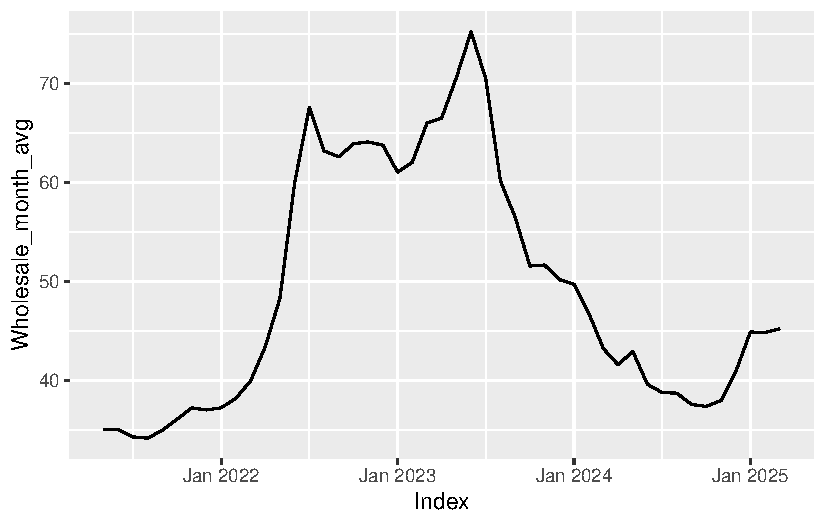
\includegraphics{Maize_analysis_files/figure-pdf/unnamed-chunk-16-1.pdf}

\subsubsection{Decomposition}\label{decomposition}

\textbf{Time series decomposition} is a technique used to break down a
time series into its key components to better understand the underlying
patterns. This is especially useful for analyzing trends, seasonality,
and irregular variations in food price data.

Types of time series decomposition we will investigate.

\begin{itemize}
\item
  \textbf{Classical decomposition}
\item
  \textbf{STL decomposition}
\item
  \textbf{X-11}
\end{itemize}

\begin{longtable}[]{@{}
  >{\raggedright\arraybackslash}p{(\columnwidth - 6\tabcolsep) * \real{0.2500}}
  >{\raggedright\arraybackslash}p{(\columnwidth - 6\tabcolsep) * \real{0.2500}}
  >{\raggedright\arraybackslash}p{(\columnwidth - 6\tabcolsep) * \real{0.2500}}
  >{\raggedright\arraybackslash}p{(\columnwidth - 6\tabcolsep) * \real{0.2500}}@{}}
\toprule\noalign{}
\begin{minipage}[b]{\linewidth}\raggedright
Method
\end{minipage} & \begin{minipage}[b]{\linewidth}\raggedright
Best For
\end{minipage} & \begin{minipage}[b]{\linewidth}\raggedright
Handles Changing Seasonality?
\end{minipage} & \begin{minipage}[b]{\linewidth}\raggedright
Handles Nonlinear Trends?
\end{minipage} \\
\midrule\noalign{}
\endhead
\bottomrule\noalign{}
\endlastfoot
Classical decomposition & Simple, regular data & ❌ No & ❌ No \\
STL decomposition & Flexible seasonality, missing data & ✅ Yes & ✅
Yes \\
X-11 & Economic data, business analysis & ✅ Yes & ✅ Yes \\
\end{longtable}

\begin{Shaded}
\begin{Highlighting}[]
\DocumentationTok{\#\# Classical decomposition}
\NormalTok{Wholesale\_ts }\OtherTok{\textless{}{-}}\FunctionTok{as.ts}\NormalTok{(Wholesale\_month\_avg)}
\FunctionTok{autoplot}\NormalTok{(}\FunctionTok{decompose}\NormalTok{(Wholesale\_ts,}\AttributeTok{type =} \StringTok{\textquotesingle{}multiplicative\textquotesingle{}}\NormalTok{)) }
\end{Highlighting}
\end{Shaded}

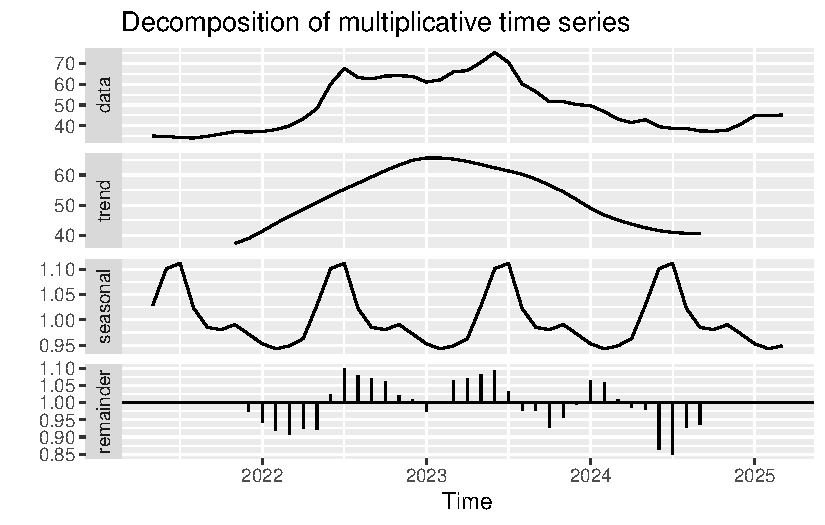
\includegraphics{Maize_analysis_files/figure-pdf/unnamed-chunk-17-1.pdf}

From decomposing the wholesale prices for maize using multiplicative
decomposition which comes in handy when there is fluctuations in the
mean prices and its is not roughly constant in size over time:

\begin{enumerate}
\def\labelenumi{\arabic{enumi}.}
\item
  The is no specific Trend in the data
\item
  Seasonality is present
\item
  In the random data their is still some patterns visible in the data
\end{enumerate}

\begin{Shaded}
\begin{Highlighting}[]
\CommentTok{\# X13}
\NormalTok{x11\_decomposed }\OtherTok{\textless{}{-}} \FunctionTok{seas}\NormalTok{(Wholesale\_ts,}\AttributeTok{x11 =} \StringTok{""}\NormalTok{)}

\FunctionTok{autoplot}\NormalTok{(x11\_decomposed)}
\end{Highlighting}
\end{Shaded}

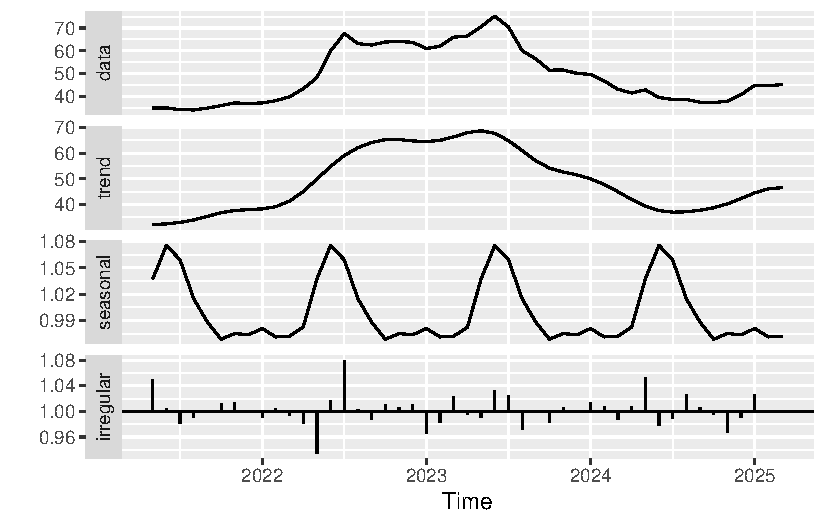
\includegraphics{Maize_analysis_files/figure-pdf/unnamed-chunk-18-1.pdf}

\begin{Shaded}
\begin{Highlighting}[]
\CommentTok{\# stl decomposition}
\NormalTok{stl\_decomposed }\OtherTok{\textless{}{-}} \FunctionTok{stl}\NormalTok{(Wholesale\_ts, }\AttributeTok{s.window =} \StringTok{"periodic"}\NormalTok{)}
\FunctionTok{autoplot}\NormalTok{(stl\_decomposed)}
\end{Highlighting}
\end{Shaded}

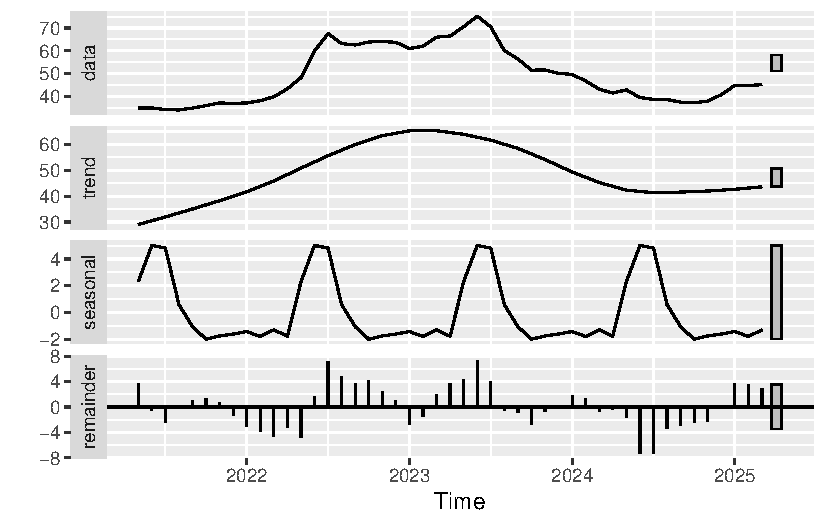
\includegraphics{Maize_analysis_files/figure-pdf/unnamed-chunk-19-1.pdf}

\subsubsection{Seasonality}\label{seasonality}

\begin{Shaded}
\begin{Highlighting}[]
\FunctionTok{ggseasonplot}\NormalTok{(Wholesale\_ts,}\AttributeTok{year.labels =} \ConstantTok{TRUE}\NormalTok{)}\SpecialCharTok{+}\FunctionTok{theme\_bw}\NormalTok{()}
\end{Highlighting}
\end{Shaded}

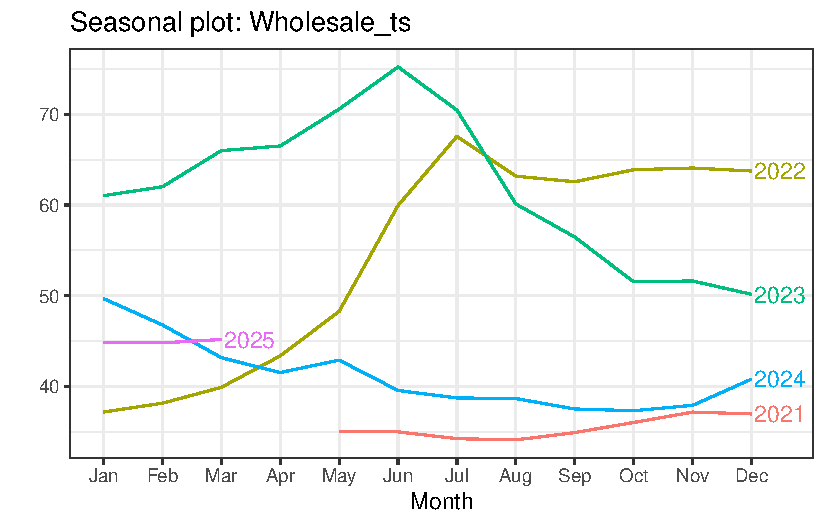
\includegraphics{Maize_analysis_files/figure-pdf/unnamed-chunk-20-1.pdf}

\subsubsection{}\label{section}

\begin{Shaded}
\begin{Highlighting}[]
\FunctionTok{ggsubseriesplot}\NormalTok{(Wholesale\_ts)}
\end{Highlighting}
\end{Shaded}

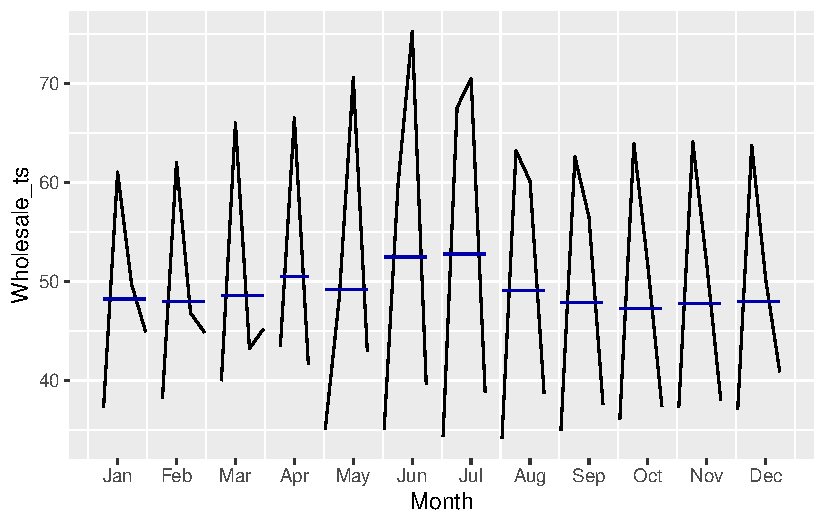
\includegraphics{Maize_analysis_files/figure-pdf/unnamed-chunk-21-1.pdf}

\begin{Shaded}
\begin{Highlighting}[]
\FunctionTok{ggtsdisplay}\NormalTok{(Wholesale\_ts,}\AttributeTok{lag.max =} \DecValTok{52}\NormalTok{)}
\end{Highlighting}
\end{Shaded}

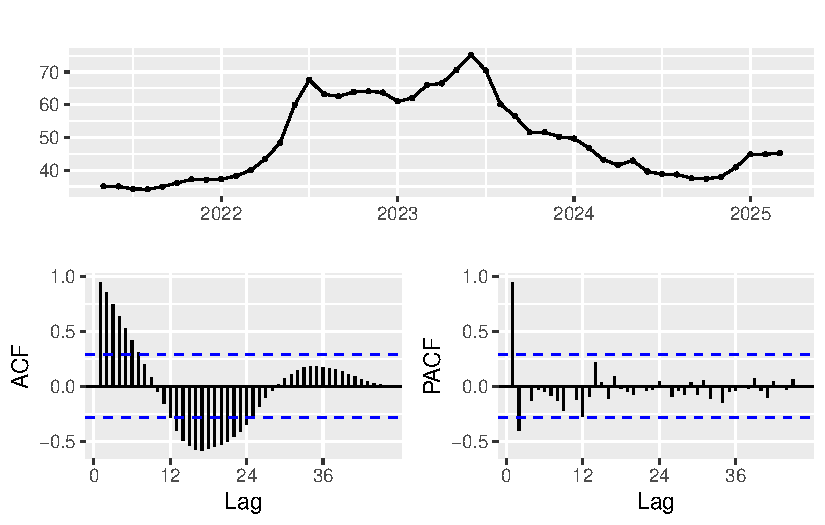
\includegraphics{Maize_analysis_files/figure-pdf/unnamed-chunk-22-1.pdf}

\subsubsection{Smoothing weekly}\label{smoothing-weekly}

\begin{Shaded}
\begin{Highlighting}[]
\NormalTok{Wholesale\_week\_avg }\OtherTok{\textless{}{-}}\FunctionTok{aggregate}\NormalTok{(Wholesale\_zoo,}\FunctionTok{floor\_date}\NormalTok{(}\FunctionTok{index}\NormalTok{(Wholesale\_zoo), }\StringTok{"week"}\NormalTok{),mean)}
\NormalTok{Wholesale\_week\_avg}
\end{Highlighting}
\end{Shaded}

\begin{verbatim}
2021-05-23 2021-05-30 2021-06-06 2021-06-13 2021-06-20 2021-06-27 2021-07-04 
  34.97000   34.32333   34.30429   35.81429   34.79714   35.02286   34.71429 
2021-07-11 2021-07-18 2021-07-25 2021-08-01 2021-08-08 2021-08-15 2021-08-22 
  34.61857   33.77857   34.42429   33.84286   34.38714   33.92429   34.69857 
2021-08-29 2021-09-05 2021-09-12 2021-09-19 2021-09-26 2021-10-03 2021-10-10 
  33.47000   34.41571   34.36286   35.85714   36.65286   35.81000   36.78571 
2021-10-17 2021-10-24 2021-10-31 2021-11-07 2021-11-14 2021-11-21 2021-11-28 
  35.06286   36.04571   36.31286   37.57857   35.68000   36.20857   39.52571 
2021-12-05 2021-12-12 2021-12-19 2021-12-26 2022-01-02 2022-01-09 2022-01-16 
  36.27143   37.54857   37.36857   36.95857   36.89286   37.10429   38.05000 
2022-01-23 2022-01-30 2022-02-06 2022-02-13 2022-02-20 2022-02-27 2022-03-06 
  37.49286   37.54286   37.93429   38.08857   38.76286   37.99857   39.34714 
2022-03-13 2022-03-20 2022-03-27 2022-04-03 2022-04-10 2022-04-17 2022-04-24 
  40.32286   40.89000   40.33143   40.87143   43.30286   44.60857   45.78000 
2022-05-01 2022-05-08 2022-05-15 2022-05-22 2022-05-29 2022-06-05 2022-06-12 
  45.99857   47.39286   49.80143   48.87286   51.60000   53.44714   57.85143 
2022-06-19 2022-06-26 2022-07-03 2022-07-10 2022-07-17 2022-07-24 2022-07-31 
  65.95429   69.93143   68.77857   69.99571   67.19857   65.24000   62.68143 
2022-08-07 2022-08-14 2022-08-21 2022-08-28 2022-09-04 2022-09-11 2022-09-18 
  63.95714   63.55857   62.47286   62.82714   61.62286   62.81571   62.86857 
2022-09-25 2022-10-02 2022-10-09 2022-10-16 2022-10-23 2022-10-30 2022-11-06 
  62.44857   64.37143   63.38000   63.74429   63.64143   65.56286   63.22857 
2022-11-13 2022-11-20 2022-11-27 2022-12-04 2022-12-11 2022-12-18 2022-12-25 
  62.91143   64.53714   64.63000   64.22429   64.00714   64.09571   61.88167 
2023-01-01 2023-01-08 2023-01-15 2023-01-22 2023-01-29 2023-02-05 2023-02-12 
  63.22000   60.42571   61.07286   59.01143   61.53143   60.34571   63.08143 
2023-02-19 2023-02-26 2023-03-05 2023-03-12 2023-03-19 2023-03-26 2023-04-02 
  62.87857   63.83143   65.27571   66.64857   65.59857   67.90143   67.23714 
2023-04-09 2023-04-16 2023-04-23 2023-04-30 2023-05-07 2023-05-14 2023-05-21 
  66.12714   66.23143   66.31714   65.83429   69.07143   70.63429   72.76286 
2023-05-28 2023-06-04 2023-06-11 2023-06-18 2023-06-25 2023-07-02 2023-07-09 
  75.00714   74.85000   76.29571   74.83857   74.86714   75.52571   72.66714 
2023-07-16 2023-07-23 2023-07-30 2023-08-06 2023-08-13 2023-08-20 2023-08-27 
  70.13714   65.36143   62.60000   62.75571   58.13571   59.74857   58.59143 
2023-09-03 2023-09-10 2023-09-17 2023-09-24 2023-10-01 2023-10-08 2023-10-15 
  57.95429   56.85286   54.57000   54.89429   52.99857   49.01571   52.97857 
2023-10-22 2023-10-29 2023-11-05 2023-11-12 2023-11-19 2023-11-26 2023-12-03 
  52.72000   49.37714   52.73714   49.62429   53.09429   51.93857   50.16857 
2023-12-10 2023-12-17 2023-12-24 2023-12-31 2024-01-07 2024-01-14 2024-01-21 
  52.39000   48.81714   49.00143   47.91800   48.10714   52.79857   50.38000 
2024-01-28 2024-02-04 2024-02-11 2024-02-18 2024-02-25 2024-03-03 2024-03-10 
  48.08143   47.39000   45.88167   46.82714   45.50500   45.20143   45.03286 
2024-03-17 2024-03-24 2024-03-31 2024-04-07 2024-04-14 2024-04-21 2024-04-28 
  41.31571   40.42286   40.94571   41.62571   39.98714   44.37833   44.10857 
2024-05-05 2024-05-12 2024-05-19 2024-05-26 2024-06-02 2024-06-09 2024-06-16 
  45.03143   42.58667   40.56333   41.31571   39.70286   40.65714   38.56714 
2024-06-23 2024-06-30 2024-07-07 2024-07-14 2024-07-21 2024-07-28 2024-08-04 
  39.85000   38.09429   39.66143   39.20857   38.33857   37.25286   40.33571 
2024-08-11 2024-08-18 2024-08-25 2024-09-01 2024-09-08 2024-09-15 2024-09-22 
  39.26000   37.00000   39.29143   37.98000   37.78000   37.61714   36.88143 
2024-09-29 2024-10-06 2024-10-13 2024-10-20 2024-10-27 2024-11-03 2024-11-10 
  36.61571   36.88857   36.41429   38.37143   37.68286   37.59571   38.04000 
2024-11-17 2024-11-24 2024-12-01 2024-12-08 2024-12-15 2024-12-22 2024-12-29 
  38.31000   38.79571   41.63857   41.06143   41.20143   39.34857   42.46833 
2025-01-05 2025-01-12 2025-01-19 2025-01-26 2025-02-02 2025-02-09 2025-02-16 
  44.87000   44.85714   46.29000   42.69286   48.03143   44.09714   43.77000 
2025-02-23 2025-03-02 2025-03-09 2025-03-16 
  44.52167   44.27714   45.56286   45.82833 
\end{verbatim}

\begin{Shaded}
\begin{Highlighting}[]
\FunctionTok{autoplot}\NormalTok{(Wholesale\_week\_avg)}
\end{Highlighting}
\end{Shaded}

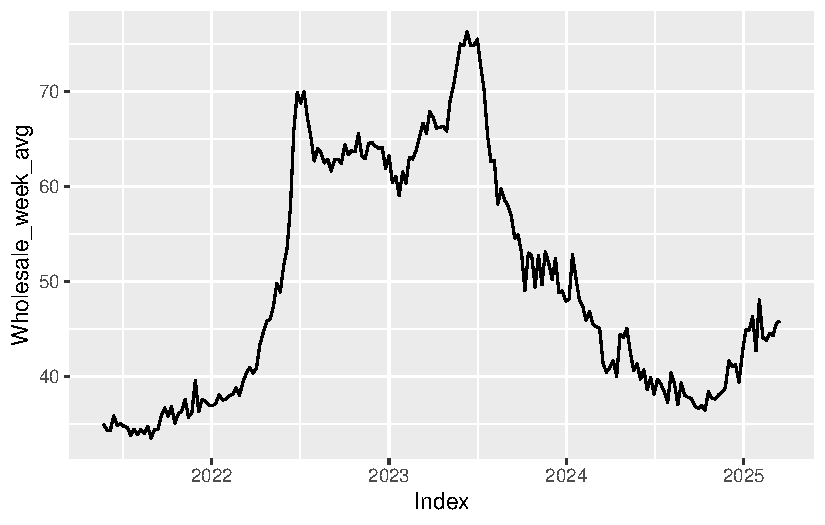
\includegraphics{Maize_analysis_files/figure-pdf/unnamed-chunk-23-1.pdf}

\paragraph{Decomposition}\label{decomposition-1}

\begin{Shaded}
\begin{Highlighting}[]
\CommentTok{\# Classical decomposition}
\NormalTok{Wholesale\_ts2 }\OtherTok{\textless{}{-}}\FunctionTok{as.ts}\NormalTok{(Wholesale\_week\_avg);Wholesale\_ts2}
\end{Highlighting}
\end{Shaded}

\begin{verbatim}
Time Series:
Start = 18770 
End = 20163 
Frequency = 0.142857142857143 
  [1] 34.97000 34.32333 34.30429 35.81429 34.79714 35.02286 34.71429 34.61857
  [9] 33.77857 34.42429 33.84286 34.38714 33.92429 34.69857 33.47000 34.41571
 [17] 34.36286 35.85714 36.65286 35.81000 36.78571 35.06286 36.04571 36.31286
 [25] 37.57857 35.68000 36.20857 39.52571 36.27143 37.54857 37.36857 36.95857
 [33] 36.89286 37.10429 38.05000 37.49286 37.54286 37.93429 38.08857 38.76286
 [41] 37.99857 39.34714 40.32286 40.89000 40.33143 40.87143 43.30286 44.60857
 [49] 45.78000 45.99857 47.39286 49.80143 48.87286 51.60000 53.44714 57.85143
 [57] 65.95429 69.93143 68.77857 69.99571 67.19857 65.24000 62.68143 63.95714
 [65] 63.55857 62.47286 62.82714 61.62286 62.81571 62.86857 62.44857 64.37143
 [73] 63.38000 63.74429 63.64143 65.56286 63.22857 62.91143 64.53714 64.63000
 [81] 64.22429 64.00714 64.09571 61.88167 63.22000 60.42571 61.07286 59.01143
 [89] 61.53143 60.34571 63.08143 62.87857 63.83143 65.27571 66.64857 65.59857
 [97] 67.90143 67.23714 66.12714 66.23143 66.31714 65.83429 69.07143 70.63429
[105] 72.76286 75.00714 74.85000 76.29571 74.83857 74.86714 75.52571 72.66714
[113] 70.13714 65.36143 62.60000 62.75571 58.13571 59.74857 58.59143 57.95429
[121] 56.85286 54.57000 54.89429 52.99857 49.01571 52.97857 52.72000 49.37714
[129] 52.73714 49.62429 53.09429 51.93857 50.16857 52.39000 48.81714 49.00143
[137] 47.91800 48.10714 52.79857 50.38000 48.08143 47.39000 45.88167 46.82714
[145] 45.50500 45.20143 45.03286 41.31571 40.42286 40.94571 41.62571 39.98714
[153] 44.37833 44.10857 45.03143 42.58667 40.56333 41.31571 39.70286 40.65714
[161] 38.56714 39.85000 38.09429 39.66143 39.20857 38.33857 37.25286 40.33571
[169] 39.26000 37.00000 39.29143 37.98000 37.78000 37.61714 36.88143 36.61571
[177] 36.88857 36.41429 38.37143 37.68286 37.59571 38.04000 38.31000 38.79571
[185] 41.63857 41.06143 41.20143 39.34857 42.46833 44.87000 44.85714 46.29000
[193] 42.69286 48.03143 44.09714 43.77000 44.52167 44.27714 45.56286 45.82833
\end{verbatim}

\begin{Shaded}
\begin{Highlighting}[]
\NormalTok{Wholesale\_ts2 }\OtherTok{\textless{}{-}} \FunctionTok{ts}\NormalTok{(Wholesale\_ts2,}\AttributeTok{frequency =} \DecValTok{52}\NormalTok{,}\AttributeTok{start =} \FunctionTok{c}\NormalTok{(}\DecValTok{2021}\NormalTok{,}\DecValTok{21}\NormalTok{));Wholesale\_ts2}
\end{Highlighting}
\end{Shaded}

\begin{verbatim}
Time Series:
Start = c(2021, 21) 
End = c(2025, 12) 
Frequency = 52 
  [1] 34.97000 34.32333 34.30429 35.81429 34.79714 35.02286 34.71429 34.61857
  [9] 33.77857 34.42429 33.84286 34.38714 33.92429 34.69857 33.47000 34.41571
 [17] 34.36286 35.85714 36.65286 35.81000 36.78571 35.06286 36.04571 36.31286
 [25] 37.57857 35.68000 36.20857 39.52571 36.27143 37.54857 37.36857 36.95857
 [33] 36.89286 37.10429 38.05000 37.49286 37.54286 37.93429 38.08857 38.76286
 [41] 37.99857 39.34714 40.32286 40.89000 40.33143 40.87143 43.30286 44.60857
 [49] 45.78000 45.99857 47.39286 49.80143 48.87286 51.60000 53.44714 57.85143
 [57] 65.95429 69.93143 68.77857 69.99571 67.19857 65.24000 62.68143 63.95714
 [65] 63.55857 62.47286 62.82714 61.62286 62.81571 62.86857 62.44857 64.37143
 [73] 63.38000 63.74429 63.64143 65.56286 63.22857 62.91143 64.53714 64.63000
 [81] 64.22429 64.00714 64.09571 61.88167 63.22000 60.42571 61.07286 59.01143
 [89] 61.53143 60.34571 63.08143 62.87857 63.83143 65.27571 66.64857 65.59857
 [97] 67.90143 67.23714 66.12714 66.23143 66.31714 65.83429 69.07143 70.63429
[105] 72.76286 75.00714 74.85000 76.29571 74.83857 74.86714 75.52571 72.66714
[113] 70.13714 65.36143 62.60000 62.75571 58.13571 59.74857 58.59143 57.95429
[121] 56.85286 54.57000 54.89429 52.99857 49.01571 52.97857 52.72000 49.37714
[129] 52.73714 49.62429 53.09429 51.93857 50.16857 52.39000 48.81714 49.00143
[137] 47.91800 48.10714 52.79857 50.38000 48.08143 47.39000 45.88167 46.82714
[145] 45.50500 45.20143 45.03286 41.31571 40.42286 40.94571 41.62571 39.98714
[153] 44.37833 44.10857 45.03143 42.58667 40.56333 41.31571 39.70286 40.65714
[161] 38.56714 39.85000 38.09429 39.66143 39.20857 38.33857 37.25286 40.33571
[169] 39.26000 37.00000 39.29143 37.98000 37.78000 37.61714 36.88143 36.61571
[177] 36.88857 36.41429 38.37143 37.68286 37.59571 38.04000 38.31000 38.79571
[185] 41.63857 41.06143 41.20143 39.34857 42.46833 44.87000 44.85714 46.29000
[193] 42.69286 48.03143 44.09714 43.77000 44.52167 44.27714 45.56286 45.82833
\end{verbatim}

\begin{Shaded}
\begin{Highlighting}[]
\FunctionTok{autoplot}\NormalTok{(}\FunctionTok{decompose}\NormalTok{(Wholesale\_ts2,}\AttributeTok{type =} \StringTok{\textquotesingle{}multiplicative\textquotesingle{}}\NormalTok{))}
\end{Highlighting}
\end{Shaded}

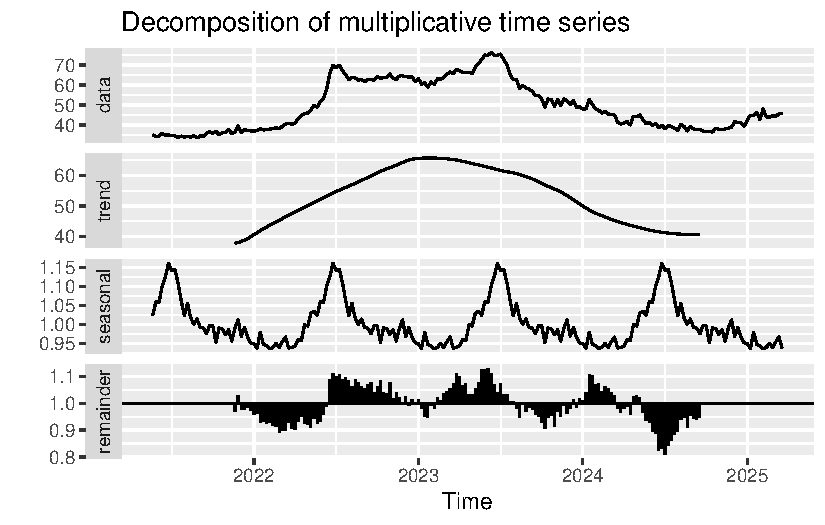
\includegraphics{Maize_analysis_files/figure-pdf/unnamed-chunk-24-1.pdf}

\begin{Shaded}
\begin{Highlighting}[]
\CommentTok{\# STL decomposition}
\FunctionTok{stl}\NormalTok{(Wholesale\_ts2,}\AttributeTok{s.window =} \StringTok{"periodic"}\NormalTok{) }\SpecialCharTok{\%\textgreater{}\%} \FunctionTok{autoplot}\NormalTok{()}
\end{Highlighting}
\end{Shaded}

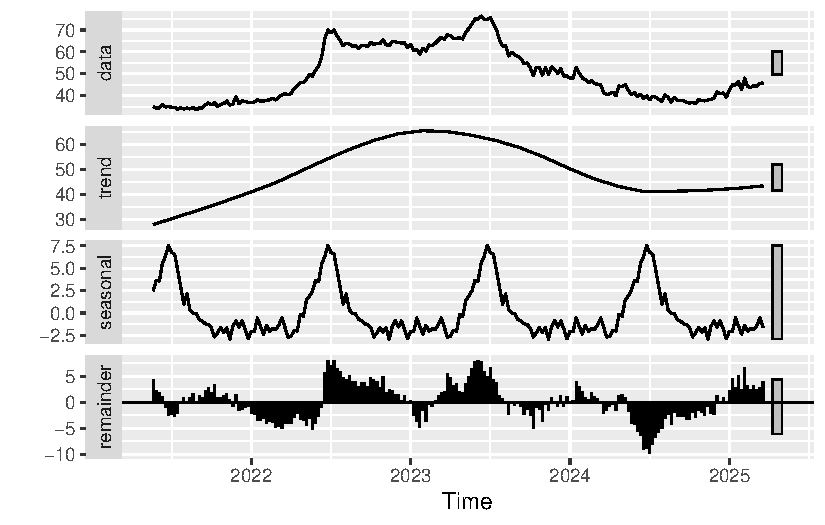
\includegraphics{Maize_analysis_files/figure-pdf/unnamed-chunk-25-1.pdf}

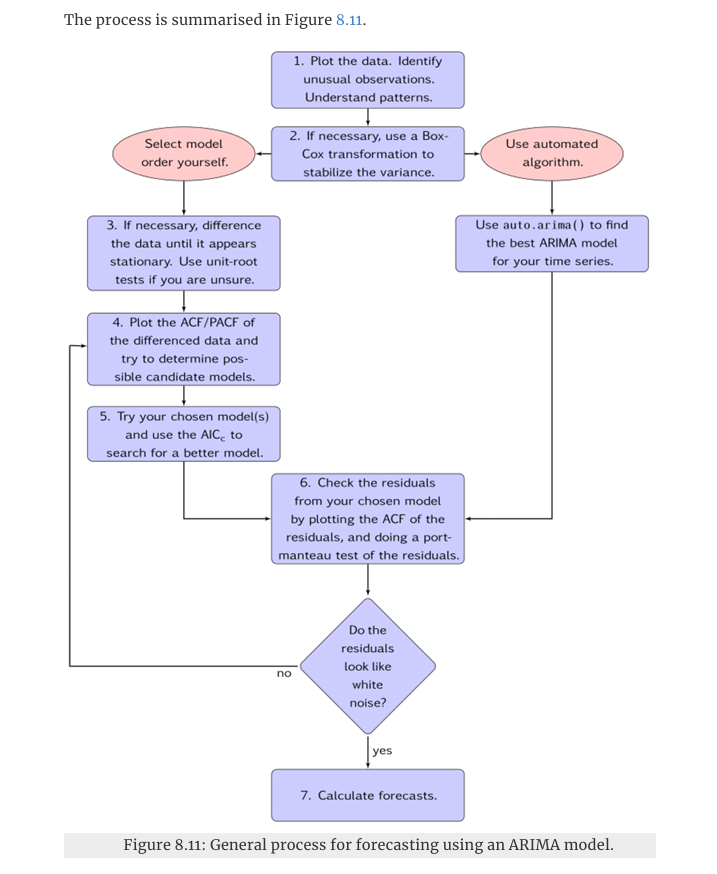
\includegraphics{images/clipboard-2535415607.png}

We will use the above strategy for Identifying an ARIMA model from
Forecasting principle Rob J Hyndman




\end{document}
